% Options for packages loaded elsewhere
\PassOptionsToPackage{unicode}{hyperref}
\PassOptionsToPackage{hyphens}{url}
%
\documentclass[
]{article}
\usepackage{lmodern}
\usepackage{amssymb,amsmath}
\usepackage{ifxetex,ifluatex}
\ifnum 0\ifxetex 1\fi\ifluatex 1\fi=0 % if pdftex
  \usepackage[T1]{fontenc}
  \usepackage[utf8]{inputenc}
  \usepackage{textcomp} % provide euro and other symbols
\else % if luatex or xetex
  \usepackage{unicode-math}
  \defaultfontfeatures{Scale=MatchLowercase}
  \defaultfontfeatures[\rmfamily]{Ligatures=TeX,Scale=1}
\fi
% Use upquote if available, for straight quotes in verbatim environments
\IfFileExists{upquote.sty}{\usepackage{upquote}}{}
\IfFileExists{microtype.sty}{% use microtype if available
  \usepackage[]{microtype}
  \UseMicrotypeSet[protrusion]{basicmath} % disable protrusion for tt fonts
}{}
\makeatletter
\@ifundefined{KOMAClassName}{% if non-KOMA class
  \IfFileExists{parskip.sty}{%
    \usepackage{parskip}
  }{% else
    \setlength{\parindent}{0pt}
    \setlength{\parskip}{6pt plus 2pt minus 1pt}}
}{% if KOMA class
  \KOMAoptions{parskip=half}}
\makeatother
\usepackage{xcolor}
\IfFileExists{xurl.sty}{\usepackage{xurl}}{} % add URL line breaks if available
\IfFileExists{bookmark.sty}{\usepackage{bookmark}}{\usepackage{hyperref}}
\hypersetup{
  pdftitle={Taller \# 3},
  pdfauthor={Julián Camilo Riaño Moreno},
  hidelinks,
  pdfcreator={LaTeX via pandoc}}
\urlstyle{same} % disable monospaced font for URLs
\usepackage[margin=1in]{geometry}
\usepackage{longtable,booktabs}
% Correct order of tables after \paragraph or \subparagraph
\usepackage{etoolbox}
\makeatletter
\patchcmd\longtable{\par}{\if@noskipsec\mbox{}\fi\par}{}{}
\makeatother
% Allow footnotes in longtable head/foot
\IfFileExists{footnotehyper.sty}{\usepackage{footnotehyper}}{\usepackage{footnote}}
\makesavenoteenv{longtable}
\usepackage{graphicx,grffile}
\makeatletter
\def\maxwidth{\ifdim\Gin@nat@width>\linewidth\linewidth\else\Gin@nat@width\fi}
\def\maxheight{\ifdim\Gin@nat@height>\textheight\textheight\else\Gin@nat@height\fi}
\makeatother
% Scale images if necessary, so that they will not overflow the page
% margins by default, and it is still possible to overwrite the defaults
% using explicit options in \includegraphics[width, height, ...]{}
\setkeys{Gin}{width=\maxwidth,height=\maxheight,keepaspectratio}
% Set default figure placement to htbp
\makeatletter
\def\fps@figure{htbp}
\makeatother
\setlength{\emergencystretch}{3em} % prevent overfull lines
\providecommand{\tightlist}{%
  \setlength{\itemsep}{0pt}\setlength{\parskip}{0pt}}
\setcounter{secnumdepth}{-\maxdimen} % remove section numbering
\usepackage{float}
\floatplacement{figure}{H}
\usepackage{booktabs}
\usepackage{longtable}
\usepackage{array}
\usepackage{multirow}
\usepackage{wrapfig}
\usepackage{float}
\usepackage{colortbl}
\usepackage{pdflscape}
\usepackage{tabu}
\usepackage{threeparttable}
\usepackage{threeparttablex}
\usepackage[normalem]{ulem}
\usepackage{makecell}
\usepackage{xcolor}

\title{Taller \# 3}
\usepackage{etoolbox}
\makeatletter
\providecommand{\subtitle}[1]{% add subtitle to \maketitle
  \apptocmd{\@title}{\par {\large #1 \par}}{}{}
}
\makeatother
\subtitle{Diagnóstico de regresión lineal múltiple}
\author{Julián Camilo Riaño Moreno}
\date{miércoles, abril 08, 2020}

\begin{document}
\maketitle

{
\setcounter{tocdepth}{3}
\tableofcontents
}
\pagebreak

\hypertarget{descripciuxf3n-de-las-variables.}{%
\section{Descripción de las
variables.}\label{descripciuxf3n-de-las-variables.}}

\begin{longtable}[]{@{}ccccc@{}}
\caption{Organizacion de las variables del taller\#3}\tabularnewline
\toprule
\begin{minipage}[b]{0.13\columnwidth}\centering
Variables dadas\strut
\end{minipage} & \begin{minipage}[b]{0.21\columnwidth}\centering
Definicion\strut
\end{minipage} & \begin{minipage}[b]{0.22\columnwidth}\centering
Tipo de variable (en modelo)\strut
\end{minipage} & \begin{minipage}[b]{0.23\columnwidth}\centering
Nombre de variable (en la base de datos)\strut
\end{minipage} & \begin{minipage}[b]{0.06\columnwidth}\centering
Unidad\strut
\end{minipage}\tabularnewline
\midrule
\endfirsthead
\toprule
\begin{minipage}[b]{0.13\columnwidth}\centering
Variables dadas\strut
\end{minipage} & \begin{minipage}[b]{0.21\columnwidth}\centering
Definicion\strut
\end{minipage} & \begin{minipage}[b]{0.22\columnwidth}\centering
Tipo de variable (en modelo)\strut
\end{minipage} & \begin{minipage}[b]{0.23\columnwidth}\centering
Nombre de variable (en la base de datos)\strut
\end{minipage} & \begin{minipage}[b]{0.06\columnwidth}\centering
Unidad\strut
\end{minipage}\tabularnewline
\midrule
\endhead
\begin{minipage}[t]{0.13\columnwidth}\centering
\(y\)\strut
\end{minipage} & \begin{minipage}[t]{0.21\columnwidth}\centering
Precio de venta de la casa\strut
\end{minipage} & \begin{minipage}[t]{0.22\columnwidth}\centering
v\_respuesta\strut
\end{minipage} & \begin{minipage}[t]{0.23\columnwidth}\centering
precioventa\strut
\end{minipage} & \begin{minipage}[t]{0.06\columnwidth}\centering
x/1000\strut
\end{minipage}\tabularnewline
\begin{minipage}[t]{0.13\columnwidth}\centering
\(x_1\)\strut
\end{minipage} & \begin{minipage}[t]{0.21\columnwidth}\centering
Impuestos (local, escuela, condado)\strut
\end{minipage} & \begin{minipage}[t]{0.22\columnwidth}\centering
v\_regresora\strut
\end{minipage} & \begin{minipage}[t]{0.23\columnwidth}\centering
impuestos\strut
\end{minipage} & \begin{minipage}[t]{0.06\columnwidth}\centering
x/1000\strut
\end{minipage}\tabularnewline
\begin{minipage}[t]{0.13\columnwidth}\centering
\(x_2\)\strut
\end{minipage} & \begin{minipage}[t]{0.21\columnwidth}\centering
Numero de banos\strut
\end{minipage} & \begin{minipage}[t]{0.22\columnwidth}\centering
v\_regresora\strut
\end{minipage} & \begin{minipage}[t]{0.23\columnwidth}\centering
num\_banos\strut
\end{minipage} & \begin{minipage}[t]{0.06\columnwidth}\centering
\(n°\)\strut
\end{minipage}\tabularnewline
\begin{minipage}[t]{0.13\columnwidth}\centering
\(x_3\)\strut
\end{minipage} & \begin{minipage}[t]{0.21\columnwidth}\centering
Tamano de lote\strut
\end{minipage} & \begin{minipage}[t]{0.22\columnwidth}\centering
v\_regresora\strut
\end{minipage} & \begin{minipage}[t]{0.23\columnwidth}\centering
tamano\_lote\strut
\end{minipage} & \begin{minipage}[t]{0.06\columnwidth}\centering
\(ft^2\)\strut
\end{minipage}\tabularnewline
\begin{minipage}[t]{0.13\columnwidth}\centering
\(x_4\)\strut
\end{minipage} & \begin{minipage}[t]{0.21\columnwidth}\centering
Espacio vital\strut
\end{minipage} & \begin{minipage}[t]{0.22\columnwidth}\centering
v\_regresora\strut
\end{minipage} & \begin{minipage}[t]{0.23\columnwidth}\centering
espac\_vital\strut
\end{minipage} & \begin{minipage}[t]{0.06\columnwidth}\centering
\(ft^2\)\strut
\end{minipage}\tabularnewline
\begin{minipage}[t]{0.13\columnwidth}\centering
\(x_5\)\strut
\end{minipage} & \begin{minipage}[t]{0.21\columnwidth}\centering
Numero de puestos de garaje\strut
\end{minipage} & \begin{minipage}[t]{0.22\columnwidth}\centering
v\_regresora\strut
\end{minipage} & \begin{minipage}[t]{0.23\columnwidth}\centering
num\_puestos\_gar\strut
\end{minipage} & \begin{minipage}[t]{0.06\columnwidth}\centering
\(n°\)\strut
\end{minipage}\tabularnewline
\begin{minipage}[t]{0.13\columnwidth}\centering
\(x_6\)\strut
\end{minipage} & \begin{minipage}[t]{0.21\columnwidth}\centering
Numero de habitaciones\strut
\end{minipage} & \begin{minipage}[t]{0.22\columnwidth}\centering
v\_regresora\strut
\end{minipage} & \begin{minipage}[t]{0.23\columnwidth}\centering
num\_hab\strut
\end{minipage} & \begin{minipage}[t]{0.06\columnwidth}\centering
\(n°\)\strut
\end{minipage}\tabularnewline
\begin{minipage}[t]{0.13\columnwidth}\centering
\(x_7\)\strut
\end{minipage} & \begin{minipage}[t]{0.21\columnwidth}\centering
Numero de dormitorios\strut
\end{minipage} & \begin{minipage}[t]{0.22\columnwidth}\centering
v\_regresora\strut
\end{minipage} & \begin{minipage}[t]{0.23\columnwidth}\centering
num\_dorm\strut
\end{minipage} & \begin{minipage}[t]{0.06\columnwidth}\centering
\(n°\)\strut
\end{minipage}\tabularnewline
\begin{minipage}[t]{0.13\columnwidth}\centering
\(x_8\)\strut
\end{minipage} & \begin{minipage}[t]{0.21\columnwidth}\centering
Edad del hogar\strut
\end{minipage} & \begin{minipage}[t]{0.22\columnwidth}\centering
v\_regresora\strut
\end{minipage} & \begin{minipage}[t]{0.23\columnwidth}\centering
edad\_hogar\strut
\end{minipage} & \begin{minipage}[t]{0.06\columnwidth}\centering
Anos\strut
\end{minipage}\tabularnewline
\begin{minipage}[t]{0.13\columnwidth}\centering
\(x_9\)\strut
\end{minipage} & \begin{minipage}[t]{0.21\columnwidth}\centering
Cantidad de chimeneas\strut
\end{minipage} & \begin{minipage}[t]{0.22\columnwidth}\centering
v\_regresora\strut
\end{minipage} & \begin{minipage}[t]{0.23\columnwidth}\centering
cant\_chimen\strut
\end{minipage} & \begin{minipage}[t]{0.06\columnwidth}\centering
\(n°\)\strut
\end{minipage}\tabularnewline
\bottomrule
\end{longtable}

En la tabla 1. se describen las caracteristicas de las variables dadas
para el ejercicio. Para ajustar las variables definidas se les asignó un
nombre para la base de datos que corresponde a la columna ``Nombre de
variable (en la base de datos)''. Además, se definió para este ejercicio
la variable respuesta \texttt{precioventa}, la cual corresponde a una
variable cuantitativa continua; las demás variables se definieron como
variables regresoras (\texttt{impuestos}, \texttt{num\_banos},
\texttt{tamano\_lote}, \texttt{espac\_vital},
\texttt{num\_puestos\_gar}, \texttt{num\_hab}, \texttt{num\_dorm},
\texttt{edad\_hogar}, \texttt{cant\_chimen}), de estas
\texttt{num\_banos}, \texttt{num\_puestos\_gar}, \texttt{num\_hab},
\texttt{num\_dorm}, \texttt{edad\_hogar}, son consideradas variables
cuantitativas discretas, las son variables cuantitativas continuas.

\begin{figure}
\centering
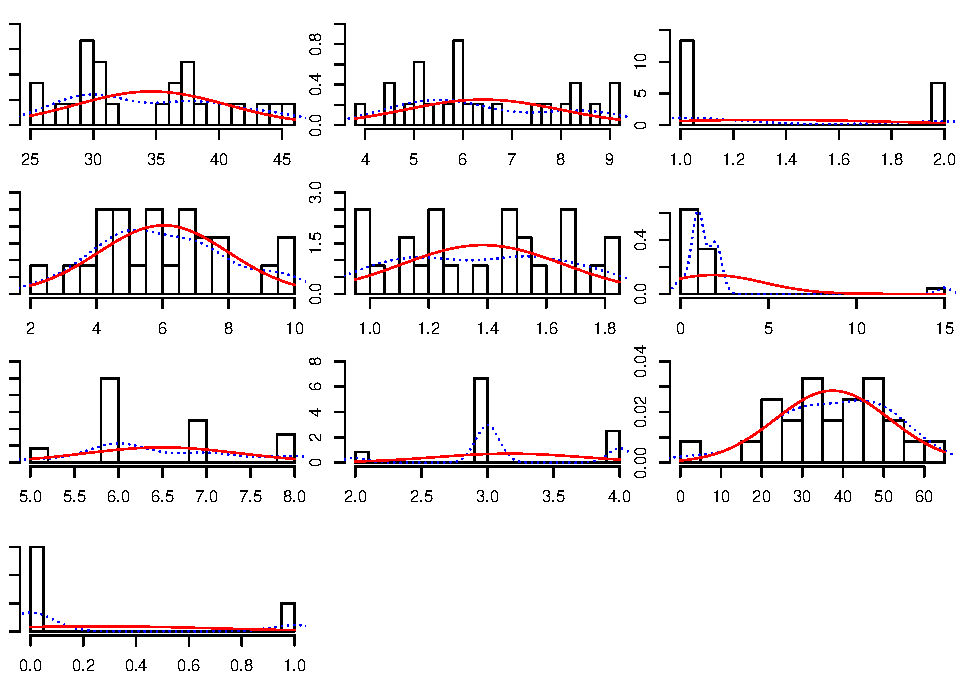
\includegraphics{diagnosticorrpp_files/figure-latex/distribuciones de las variables dadas-1.pdf}
\caption{Distribución de las variables dadas}
\end{figure}

La figura 1, muestra la distribución de las 9 variables que serán
análizadas en este documento. En esta figura se deja ver que la variable
\texttt{num\_banos} (\(x_2\)) al igual que la variable
\texttt{cant\_chimen} presentan múltiples datos extremos. Las demás
variables presenta una distribución normal.

\hypertarget{respuesta-a-la-preguntas-taller-3}{%
\section{Respuesta a la preguntas taller \#
3}\label{respuesta-a-la-preguntas-taller-3}}

\hypertarget{problema}{%
\subsection{Problema}\label{problema}}

Considere los datos de precios de la vivienda dados en la tabla 1. a.
Ajuste un modelo de regresióon múultiple que relacione el precio de
venta con los nueve regresores. segundo. Prueba de signifícación de la
regresión. ¿Qué conclusiones puedes sacar?. Utilice las pruebas t para
evaluar la contribución de cada regresor al modelo. Discute tus
hallazgos.

\hypertarget{pregunta-1-ajuste-un-modelo-de-regresiuxf3n-muxfaltiple-que-relacione-el-precio-de-venta-con-los-nueve-variables-regresoras.}{%
\subsubsection{Pregunta \#1: Ajuste un modelo de regresión múltiple que
relacione el precio de venta con los nueve variables
regresoras.}\label{pregunta-1-ajuste-un-modelo-de-regresiuxf3n-muxfaltiple-que-relacione-el-precio-de-venta-con-los-nueve-variables-regresoras.}}

\begin{figure}
\centering
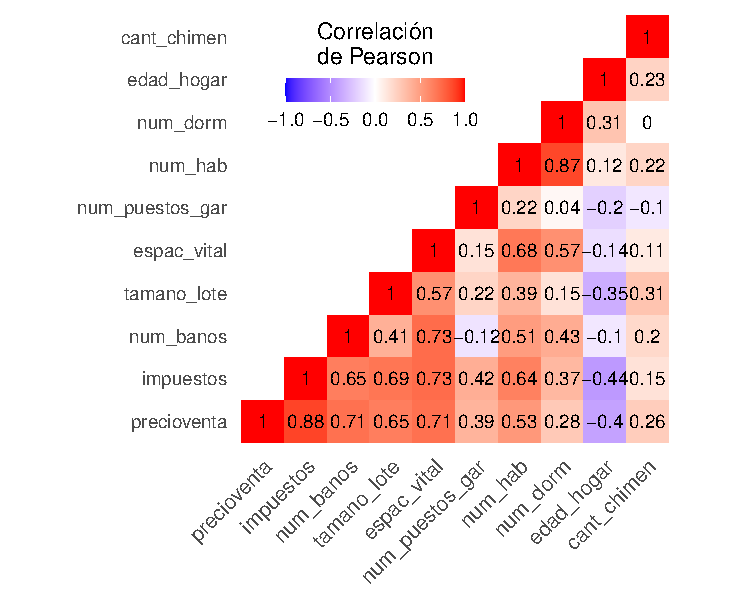
\includegraphics{diagnosticorrpp_files/figure-latex/heat map de correlaciones con ggcorrplot-1.pdf}
\caption{Mapa de calor de correlaciones entre variables}
\end{figure}

Inicialmente se realizó un análisis de correlación de las variables
dadas por medio del coeficiente de correlación de Pearson (coeficientes
mostrados en la figura 2). A través de este examen se encontró que la
variable regresora \texttt{impuestos} (cor=0.81) es la más
correlacionada con la variable respuesta \texttt{precioventa}. Otras
variables con alta correlación con la variable respuesta fueron,
\texttt{num\_banos} y \texttt{espac\_vital} (cor=0.71), seguidas de
\texttt{tamano\_lote}(cor=0.65). Entre las variables regresoras se
encuentran alta correlación entre \texttt{num\_hab} y \texttt{num\_dorm}
(cor=0.87), seguidas de \texttt{espac\_vital} con \texttt{num\_banos} e
\texttt{Impuestos}(cor=0.73). Las variables con menor correlación son
\texttt{num\_dorm} con \texttt{cant\_chimen} y
\texttt{num\_puestos\_gar}con \texttt{num\_dorm}.

\hypertarget{pregunta-2-prueba-de-signicancia-de-la-regresiuxf3n.-quuxe9-conclusiones-puedes-sacar}{%
\subsubsection{Pregunta \#2: Prueba de signicancia de la regresión. ¿Qué
conclusiones puedes
sacar?}\label{pregunta-2-prueba-de-signicancia-de-la-regresiuxf3n.-quuxe9-conclusiones-puedes-sacar}}

Se elaboró un modelo de regresión original realizado entre las variable
respuesta \texttt{precioventa} y las otras nueve variables regresoras.
Para evaluar el modelo, se realizó un análisis de la \(F\) de Fisher
para el modelo que llamaremos original con 9 variable y un análisis de
\(R_{adj}^2\).

\begin{longtable}[]{@{}ccc@{}}
\caption{Estadistico \(F\) de Fisher: significancia del
modelo}\tabularnewline
\toprule
\begin{minipage}[b]{0.24\columnwidth}\centering
\(F_{stat}\)\strut
\end{minipage} & \begin{minipage}[b]{0.23\columnwidth}\centering
Grados\_libertad\strut
\end{minipage} & \begin{minipage}[b]{0.15\columnwidth}\centering
\(p-value\)\strut
\end{minipage}\tabularnewline
\midrule
\endfirsthead
\toprule
\begin{minipage}[b]{0.24\columnwidth}\centering
\(F_{stat}\)\strut
\end{minipage} & \begin{minipage}[b]{0.23\columnwidth}\centering
Grados\_libertad\strut
\end{minipage} & \begin{minipage}[b]{0.15\columnwidth}\centering
\(p-value\)\strut
\end{minipage}\tabularnewline
\midrule
\endhead
\begin{minipage}[t]{0.24\columnwidth}\centering
10.5619486137295\strut
\end{minipage} & \begin{minipage}[t]{0.23\columnwidth}\centering
14\strut
\end{minipage} & \begin{minipage}[t]{0.15\columnwidth}\centering
7.694e-05\strut
\end{minipage}\tabularnewline
\bottomrule
\end{longtable}

En la tabla 2. se encuentran los resultado de \(F\) de fisher, para el
análisis de la siguiente prueba de hipotesis:

\[
H_o: \beta_1 = \beta_2 =  ... =\beta_k = 0 \\ 
\]

\[
H_1: \beta_j \neq 0 \ para \ cualquier  \ j \ dado
\]

El estadístico \(F\) de Fisher se obtuvo con 14 grados de libertad,
donde el \(p-value\) demuestra significancia estadística, con lo que se
rechaza la hipotesis nula. De tal forma, se puede inferir que almenos
una de la variables regresoras (\(\beta_i\)) son diferentes de 0.

\begin{longtable}[]{@{}cc@{}}
\caption{\(R^2\) y \(R_{adj}^2\) para el modelo}\tabularnewline
\toprule
\begin{minipage}[b]{0.10\columnwidth}\centering
\(R^2\)\strut
\end{minipage} & \begin{minipage}[b]{0.18\columnwidth}\centering
\(R_{adj}^2\)\strut
\end{minipage}\tabularnewline
\midrule
\endfirsthead
\toprule
\begin{minipage}[b]{0.10\columnwidth}\centering
\(R^2\)\strut
\end{minipage} & \begin{minipage}[b]{0.18\columnwidth}\centering
\(R_{adj}^2\)\strut
\end{minipage}\tabularnewline
\midrule
\endhead
\begin{minipage}[t]{0.10\columnwidth}\centering
0.872\strut
\end{minipage} & \begin{minipage}[t]{0.18\columnwidth}\centering
0.789\strut
\end{minipage}\tabularnewline
\bottomrule
\end{longtable}

Por otra parte, la tabla 3, muestra los resultados de los \(R^2\) y
\(R_{adj}^2\) para el modelo de regresión original. Estos resultados
(\(R^2 \neq R_{adj}^2\)). Para el análisis se tendrá en cuenta el
\(R_{adj}^2\) ya que es el menos sensible a la supresión o adición de
variables.De manera que este resultado, permiten inferir que
aproximadamente el 79\% de la variabilidad de la variable respuesta
(\texttt{precioventa}) puede ser explicado por las variables regresoras
de este modelo; de manera que, la variabilidad restante puede ser
consecuencia a otras variables no tenidas encuenta en el modelo o por
azar.

\begin{longtable}[]{@{}ccc@{}}
\caption{Intervalos de confianza del 95\% para los parametros del modelo
original}\tabularnewline
\toprule
\begin{minipage}[b]{0.28\columnwidth}\centering
~\strut
\end{minipage} & \begin{minipage}[b]{0.14\columnwidth}\centering
IC 2.5\%\strut
\end{minipage} & \begin{minipage}[b]{0.14\columnwidth}\centering
IC 97.5\%\strut
\end{minipage}\tabularnewline
\midrule
\endfirsthead
\toprule
\begin{minipage}[b]{0.28\columnwidth}\centering
~\strut
\end{minipage} & \begin{minipage}[b]{0.14\columnwidth}\centering
IC 2.5\%\strut
\end{minipage} & \begin{minipage}[b]{0.14\columnwidth}\centering
IC 97.5\%\strut
\end{minipage}\tabularnewline
\midrule
\endhead
\begin{minipage}[t]{0.28\columnwidth}\centering
\textbf{precioventa}\strut
\end{minipage} & \begin{minipage}[t]{0.14\columnwidth}\centering
8.67\strut
\end{minipage} & \begin{minipage}[t]{0.14\columnwidth}\centering
31.8\strut
\end{minipage}\tabularnewline
\begin{minipage}[t]{0.28\columnwidth}\centering
\textbf{impuestos}\strut
\end{minipage} & \begin{minipage}[t]{0.14\columnwidth}\centering
-1.04\strut
\end{minipage} & \begin{minipage}[t]{0.14\columnwidth}\centering
3.53\strut
\end{minipage}\tabularnewline
\begin{minipage}[t]{0.28\columnwidth}\centering
\textbf{num\_banos}\strut
\end{minipage} & \begin{minipage}[t]{0.14\columnwidth}\centering
0.345\strut
\end{minipage} & \begin{minipage}[t]{0.14\columnwidth}\centering
10.1\strut
\end{minipage}\tabularnewline
\begin{minipage}[t]{0.28\columnwidth}\centering
\textbf{tamano\_lote}\strut
\end{minipage} & \begin{minipage}[t]{0.14\columnwidth}\centering
-0.823\strut
\end{minipage} & \begin{minipage}[t]{0.14\columnwidth}\centering
1.13\strut
\end{minipage}\tabularnewline
\begin{minipage}[t]{0.28\columnwidth}\centering
\textbf{espac\_vital}\strut
\end{minipage} & \begin{minipage}[t]{0.14\columnwidth}\centering
-6.83\strut
\end{minipage} & \begin{minipage}[t]{0.14\columnwidth}\centering
10.6\strut
\end{minipage}\tabularnewline
\begin{minipage}[t]{0.28\columnwidth}\centering
\textbf{num\_puestos\_gar}\strut
\end{minipage} & \begin{minipage}[t]{0.14\columnwidth}\centering
-0.00951\strut
\end{minipage} & \begin{minipage}[t]{0.14\columnwidth}\centering
1.21\strut
\end{minipage}\tabularnewline
\begin{minipage}[t]{0.28\columnwidth}\centering
\textbf{num\_hab}\strut
\end{minipage} & \begin{minipage}[t]{0.14\columnwidth}\centering
-5.69\strut
\end{minipage} & \begin{minipage}[t]{0.14\columnwidth}\centering
3.86\strut
\end{minipage}\tabularnewline
\begin{minipage}[t]{0.28\columnwidth}\centering
\textbf{num\_dorm}\strut
\end{minipage} & \begin{minipage}[t]{0.14\columnwidth}\centering
-5.67\strut
\end{minipage} & \begin{minipage}[t]{0.14\columnwidth}\centering
7.52\strut
\end{minipage}\tabularnewline
\begin{minipage}[t]{0.28\columnwidth}\centering
\textbf{edad\_hogar}\strut
\end{minipage} & \begin{minipage}[t]{0.14\columnwidth}\centering
-0.215\strut
\end{minipage} & \begin{minipage}[t]{0.14\columnwidth}\centering
0.0598\strut
\end{minipage}\tabularnewline
\begin{minipage}[t]{0.28\columnwidth}\centering
\textbf{cant\_chimen}\strut
\end{minipage} & \begin{minipage}[t]{0.14\columnwidth}\centering
-1.12\strut
\end{minipage} & \begin{minipage}[t]{0.14\columnwidth}\centering
6.66\strut
\end{minipage}\tabularnewline
\bottomrule
\end{longtable}

La tabla 4. muestra los intervalos de confianza para los parametros del
modelo original, destacándose la amplitud encontrada resultadas para las
variables \texttt{cant\_chimen}, \texttt{num\_dorm} y \texttt{num\_hab}.

\hypertarget{pregunta-3-utilice-las-pruebas-t-para-evaluar-la-contribuciuxf3n-de-cada-variable-regresora-al-modelo.-discute-tus-hallazgos.}{%
\subsubsection{Pregunta \#3: Utilice las pruebas t para evaluar la
contribución de cada variable regresora al modelo. Discute tus
hallazgos.}\label{pregunta-3-utilice-las-pruebas-t-para-evaluar-la-contribuciuxf3n-de-cada-variable-regresora-al-modelo.-discute-tus-hallazgos.}}

\begin{longtable}[]{@{}ccccc@{}}
\caption{Estimaciones y \(t-values\) para el modelo
obtenido}\tabularnewline
\toprule
\begin{minipage}[b]{0.26\columnwidth}\centering
~\strut
\end{minipage} & \begin{minipage}[b]{0.13\columnwidth}\centering
Estimado\strut
\end{minipage} & \begin{minipage}[b]{0.16\columnwidth}\centering
ErrorStand\strut
\end{minipage} & \begin{minipage}[b]{0.14\columnwidth}\centering
\(t-value\)\strut
\end{minipage} & \begin{minipage}[b]{0.14\columnwidth}\centering
\(p-value\)\strut
\end{minipage}\tabularnewline
\midrule
\endfirsthead
\toprule
\begin{minipage}[b]{0.26\columnwidth}\centering
~\strut
\end{minipage} & \begin{minipage}[b]{0.13\columnwidth}\centering
Estimado\strut
\end{minipage} & \begin{minipage}[b]{0.16\columnwidth}\centering
ErrorStand\strut
\end{minipage} & \begin{minipage}[b]{0.14\columnwidth}\centering
\(t-value\)\strut
\end{minipage} & \begin{minipage}[b]{0.14\columnwidth}\centering
\(p-value\)\strut
\end{minipage}\tabularnewline
\midrule
\endhead
\begin{minipage}[t]{0.26\columnwidth}\centering
\textbf{(Intercept)}\strut
\end{minipage} & \begin{minipage}[t]{0.13\columnwidth}\centering
20.2\strut
\end{minipage} & \begin{minipage}[t]{0.16\columnwidth}\centering
5.39\strut
\end{minipage} & \begin{minipage}[t]{0.14\columnwidth}\centering
3.75\strut
\end{minipage} & \begin{minipage}[t]{0.14\columnwidth}\centering
0.00214\strut
\end{minipage}\tabularnewline
\begin{minipage}[t]{0.26\columnwidth}\centering
\textbf{impuestos}\strut
\end{minipage} & \begin{minipage}[t]{0.13\columnwidth}\centering
1.25\strut
\end{minipage} & \begin{minipage}[t]{0.16\columnwidth}\centering
1.06\strut
\end{minipage} & \begin{minipage}[t]{0.14\columnwidth}\centering
1.17\strut
\end{minipage} & \begin{minipage}[t]{0.14\columnwidth}\centering
0.262\strut
\end{minipage}\tabularnewline
\begin{minipage}[t]{0.26\columnwidth}\centering
\textbf{num\_banos}\strut
\end{minipage} & \begin{minipage}[t]{0.13\columnwidth}\centering
5.23\strut
\end{minipage} & \begin{minipage}[t]{0.16\columnwidth}\centering
2.28\strut
\end{minipage} & \begin{minipage}[t]{0.14\columnwidth}\centering
2.3\strut
\end{minipage} & \begin{minipage}[t]{0.14\columnwidth}\centering
0.0376\strut
\end{minipage}\tabularnewline
\begin{minipage}[t]{0.26\columnwidth}\centering
\textbf{tamano\_lote}\strut
\end{minipage} & \begin{minipage}[t]{0.13\columnwidth}\centering
0.156\strut
\end{minipage} & \begin{minipage}[t]{0.16\columnwidth}\centering
0.456\strut
\end{minipage} & \begin{minipage}[t]{0.14\columnwidth}\centering
0.341\strut
\end{minipage} & \begin{minipage}[t]{0.14\columnwidth}\centering
0.738\strut
\end{minipage}\tabularnewline
\begin{minipage}[t]{0.26\columnwidth}\centering
\textbf{espac\_vital}\strut
\end{minipage} & \begin{minipage}[t]{0.13\columnwidth}\centering
1.89\strut
\end{minipage} & \begin{minipage}[t]{0.16\columnwidth}\centering
4.07\strut
\end{minipage} & \begin{minipage}[t]{0.14\columnwidth}\centering
0.466\strut
\end{minipage} & \begin{minipage}[t]{0.14\columnwidth}\centering
0.649\strut
\end{minipage}\tabularnewline
\begin{minipage}[t]{0.26\columnwidth}\centering
\textbf{num\_puestos\_gar}\strut
\end{minipage} & \begin{minipage}[t]{0.13\columnwidth}\centering
0.598\strut
\end{minipage} & \begin{minipage}[t]{0.16\columnwidth}\centering
0.283\strut
\end{minipage} & \begin{minipage}[t]{0.14\columnwidth}\centering
2.11\strut
\end{minipage} & \begin{minipage}[t]{0.14\columnwidth}\centering
0.0532\strut
\end{minipage}\tabularnewline
\begin{minipage}[t]{0.26\columnwidth}\centering
\textbf{num\_hab}\strut
\end{minipage} & \begin{minipage}[t]{0.13\columnwidth}\centering
-0.914\strut
\end{minipage} & \begin{minipage}[t]{0.16\columnwidth}\centering
2.23\strut
\end{minipage} & \begin{minipage}[t]{0.14\columnwidth}\centering
-0.41\strut
\end{minipage} & \begin{minipage}[t]{0.14\columnwidth}\centering
0.688\strut
\end{minipage}\tabularnewline
\begin{minipage}[t]{0.26\columnwidth}\centering
\textbf{num\_dorm}\strut
\end{minipage} & \begin{minipage}[t]{0.13\columnwidth}\centering
0.926\strut
\end{minipage} & \begin{minipage}[t]{0.16\columnwidth}\centering
3.07\strut
\end{minipage} & \begin{minipage}[t]{0.14\columnwidth}\centering
0.301\strut
\end{minipage} & \begin{minipage}[t]{0.14\columnwidth}\centering
0.768\strut
\end{minipage}\tabularnewline
\begin{minipage}[t]{0.26\columnwidth}\centering
\textbf{edad\_hogar}\strut
\end{minipage} & \begin{minipage}[t]{0.13\columnwidth}\centering
-0.0775\strut
\end{minipage} & \begin{minipage}[t]{0.16\columnwidth}\centering
0.0641\strut
\end{minipage} & \begin{minipage}[t]{0.14\columnwidth}\centering
-1.21\strut
\end{minipage} & \begin{minipage}[t]{0.14\columnwidth}\centering
0.246\strut
\end{minipage}\tabularnewline
\begin{minipage}[t]{0.26\columnwidth}\centering
\textbf{cant\_chimen}\strut
\end{minipage} & \begin{minipage}[t]{0.13\columnwidth}\centering
2.77\strut
\end{minipage} & \begin{minipage}[t]{0.16\columnwidth}\centering
1.81\strut
\end{minipage} & \begin{minipage}[t]{0.14\columnwidth}\centering
1.53\strut
\end{minipage} & \begin{minipage}[t]{0.14\columnwidth}\centering
0.149\strut
\end{minipage}\tabularnewline
\bottomrule
\end{longtable}

Los resultados mostrados en la tabla 5, donde se muestran las
estimaciones del modelo original y sus \(t-values\), muestran un
estimado del intercepto (\texttt{precioventa}) un valor positivo \(> 0\)
(20.2); de manera que de estos resultados se puede deducir que algunos
estimadores de las variables regresoras, pueden afectar el resultado de
la variable respuesta. Al verificar los \(t-values\) se observa que solo
son significativas \texttt{num\_banos} (\(p - value < 0.05\)). Las demás
variables regresoras no son significativas (\(p - value \geq 0.05\))
para establecer su efecto sobre la variable respuesta en el modelo
original. Con este modelo en una interpretación prudente solo es posible
afirmar que un incremento en una unidad del numero de baños se puede
incrementar 5.23/1000 dolares el precio de venta de la propiedad,
siempre que las otras variables no cambien.

\hypertarget{pregunta-4-ajuste-un-nuevo-modelo-lineal-que-contenga-suxf3lo-las-variables-regresoras-que-resultaron-signifuxedcativas-en-la-prueba-anterior.}{%
\subsubsection{Pregunta \#4: Ajuste un nuevo modelo lineal que contenga
sólo las variables regresoras que resultaron signifícativas en la prueba
anterior.}\label{pregunta-4-ajuste-un-nuevo-modelo-lineal-que-contenga-suxf3lo-las-variables-regresoras-que-resultaron-signifuxedcativas-en-la-prueba-anterior.}}

Dado los resultados anteriores se decide realizar un ajuste del modelo
aplicando el método \emph{stepwise} y aplicando los estadisticos
\(AIC\), \(BIC\), \(Cp\) y \(R^2_{adj}\).

Le método \(AIC\) (Akaike) fue realizado a través de la función
\texttt{step}, con un método \emph{stepwise} bidireccional
\emph{forward} y \emph{reverse}, a partir de esta estratégia se obtuvo
que el \textbf{``mejor modelo''} sería uno que incluyera únicamente 5
variables regresoras, a saber: \texttt{impuestos}, \texttt{num\_banos},
\texttt{num\_puestos\_gar}, \texttt{edad\_hogar}, \texttt{cant\_chimen}.

\begin{figure}
\centering
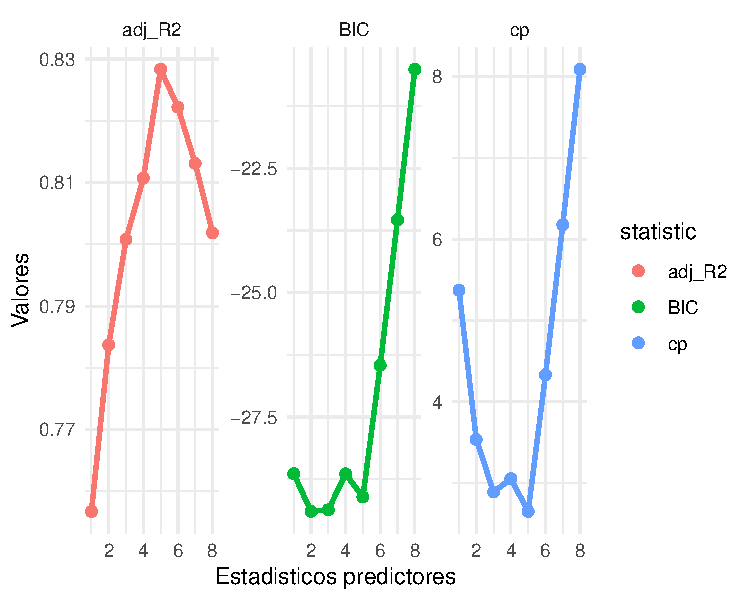
\includegraphics{diagnosticorrpp_files/figure-latex/Gráfica de ESTADISTICOS para elección de mejor modelo-1.pdf}
\caption{Estadísticos para elección de mejor modelo: adj\_R2, BIC, Cp}
\end{figure}

Además se realizó un análisis utilizando otros estadisticos bajo el
método \emph{stepwise} para este caso se utilizó unicamente un
direccionamiento \emph{forward} o de introducción progresiva, con estas
precisiones los resultados fueron similares al \(AIC\) como se puede ver
en la figura 3. Es de notar que Para el método \(R^2_{adj}\) y \(Cp\)
muestran que el mejor modelo es el \#5 que corresponde al mismo modelo
obtenido por \(AIC\). No obstante, estadistico \(BIC\) muestra que el
mejor modelo es el \#2 esto es: \texttt{impuestos} y
\texttt{num\_banos}. Para efectos del desarrollo de esta actividad se
tomará el modelo de 5 (que será designado como ``\emph{mejor modelo}'')
variables por la consistencia de resultados en los demás estadísticos.

\hypertarget{pregunta-5-interprete-los-paruxe1metros-estimados-del-nuevo-modelo.}{%
\subsubsection{Pregunta \#5: Interprete los parámetros estimados del
nuevo
modelo.}\label{pregunta-5-interprete-los-paruxe1metros-estimados-del-nuevo-modelo.}}

\begin{longtable}[]{@{}ccccc@{}}
\caption{Estimadores, \(t-values\) y significancia para el mejor modelo
sugerido por AIC, Cp, y \(r^2_{adj}\)}\tabularnewline
\toprule
\begin{minipage}[b]{0.26\columnwidth}\centering
~\strut
\end{minipage} & \begin{minipage}[b]{0.13\columnwidth}\centering
Estimado\strut
\end{minipage} & \begin{minipage}[b]{0.16\columnwidth}\centering
ErrorStand\strut
\end{minipage} & \begin{minipage}[b]{0.14\columnwidth}\centering
\(t-value\)\strut
\end{minipage} & \begin{minipage}[b]{0.14\columnwidth}\centering
\(p-value\)\strut
\end{minipage}\tabularnewline
\midrule
\endfirsthead
\toprule
\begin{minipage}[b]{0.26\columnwidth}\centering
~\strut
\end{minipage} & \begin{minipage}[b]{0.13\columnwidth}\centering
Estimado\strut
\end{minipage} & \begin{minipage}[b]{0.16\columnwidth}\centering
ErrorStand\strut
\end{minipage} & \begin{minipage}[b]{0.14\columnwidth}\centering
\(t-value\)\strut
\end{minipage} & \begin{minipage}[b]{0.14\columnwidth}\centering
\(p-value\)\strut
\end{minipage}\tabularnewline
\midrule
\endhead
\begin{minipage}[t]{0.26\columnwidth}\centering
\textbf{(Intercept)}\strut
\end{minipage} & \begin{minipage}[t]{0.13\columnwidth}\centering
19.7\strut
\end{minipage} & \begin{minipage}[t]{0.16\columnwidth}\centering
3.75\strut
\end{minipage} & \begin{minipage}[t]{0.14\columnwidth}\centering
5.24\strut
\end{minipage} & \begin{minipage}[t]{0.14\columnwidth}\centering
5.54e-05\strut
\end{minipage}\tabularnewline
\begin{minipage}[t]{0.26\columnwidth}\centering
\textbf{impuestos}\strut
\end{minipage} & \begin{minipage}[t]{0.13\columnwidth}\centering
1.35\strut
\end{minipage} & \begin{minipage}[t]{0.16\columnwidth}\centering
0.675\strut
\end{minipage} & \begin{minipage}[t]{0.14\columnwidth}\centering
1.99\strut
\end{minipage} & \begin{minipage}[t]{0.14\columnwidth}\centering
0.0617\strut
\end{minipage}\tabularnewline
\begin{minipage}[t]{0.26\columnwidth}\centering
\textbf{num\_banos}\strut
\end{minipage} & \begin{minipage}[t]{0.13\columnwidth}\centering
5.7\strut
\end{minipage} & \begin{minipage}[t]{0.16\columnwidth}\centering
1.82\strut
\end{minipage} & \begin{minipage}[t]{0.14\columnwidth}\centering
3.13\strut
\end{minipage} & \begin{minipage}[t]{0.14\columnwidth}\centering
0.00574\strut
\end{minipage}\tabularnewline
\begin{minipage}[t]{0.26\columnwidth}\centering
\textbf{num\_puestos\_gar}\strut
\end{minipage} & \begin{minipage}[t]{0.13\columnwidth}\centering
0.575\strut
\end{minipage} & \begin{minipage}[t]{0.16\columnwidth}\centering
0.25\strut
\end{minipage} & \begin{minipage}[t]{0.14\columnwidth}\centering
2.3\strut
\end{minipage} & \begin{minipage}[t]{0.14\columnwidth}\centering
0.0338\strut
\end{minipage}\tabularnewline
\begin{minipage}[t]{0.26\columnwidth}\centering
\textbf{edad\_hogar}\strut
\end{minipage} & \begin{minipage}[t]{0.13\columnwidth}\centering
-0.0787\strut
\end{minipage} & \begin{minipage}[t]{0.16\columnwidth}\centering
0.0458\strut
\end{minipage} & \begin{minipage}[t]{0.14\columnwidth}\centering
-1.72\strut
\end{minipage} & \begin{minipage}[t]{0.14\columnwidth}\centering
0.103\strut
\end{minipage}\tabularnewline
\begin{minipage}[t]{0.26\columnwidth}\centering
\textbf{cant\_chimen}\strut
\end{minipage} & \begin{minipage}[t]{0.13\columnwidth}\centering
2.54\strut
\end{minipage} & \begin{minipage}[t]{0.16\columnwidth}\centering
1.28\strut
\end{minipage} & \begin{minipage}[t]{0.14\columnwidth}\centering
1.98\strut
\end{minipage} & \begin{minipage}[t]{0.14\columnwidth}\centering
0.0628\strut
\end{minipage}\tabularnewline
\bottomrule
\end{longtable}

La tabla 6 muestra las estimaciones del ``mejor modelo'' y sus
\(t-values\), muestran un estimado del intercepto (\texttt{precioventa})
con valor positivo \(> 0\) (19.7); de manera que de estos resultados se
puede deducir que algunos estimadores de las variables regresoras,
pueden afectar el resultado de la variable respuesta. Al verificar los
\(t-values\) se observa que solo son significativas nuevamente
\texttt{num\_banos} y \texttt{num\_puestos\_gar} (\(p - value < 0.05\)).
Las demás variables regresoras utilizadas en este modelo no son
significativas (\(p - value \geq 0.05\)), por lo tanto, no es posible
establecer que puedan tener efecto alguno sobre la variable respuesta.
De acá se se puede inferir que un incremento en una unidad del numero de
baños se puede incrementar 5.7/1000 dolares el precio de venta de la
propiedad siempre que las otras variables no cambien y/o que un
incremento en una unidad del numero de puestos de garaje se puede
incrementar 0.575/1000 dolares el precio de venta de la propiedad, de
igual manera siempre que las otras variables no cambien.

\begin{longtable}[]{@{}ccc@{}}
\caption{Estadistico \(F\) de Fisher: significancia del mejor modelo Al
probar la significancia del ``mejor modelo'' se estableción nuevamente
una prueba de hipotesis de la siguiente manera:}\tabularnewline
\toprule
\begin{minipage}[b]{0.24\columnwidth}\centering
\(F_{stat}\)\strut
\end{minipage} & \begin{minipage}[b]{0.23\columnwidth}\centering
Grados\_libertad\strut
\end{minipage} & \begin{minipage}[b]{0.15\columnwidth}\centering
\(p-value\)\strut
\end{minipage}\tabularnewline
\midrule
\endfirsthead
\toprule
\begin{minipage}[b]{0.24\columnwidth}\centering
\(F_{stat}\)\strut
\end{minipage} & \begin{minipage}[b]{0.23\columnwidth}\centering
Grados\_libertad\strut
\end{minipage} & \begin{minipage}[b]{0.15\columnwidth}\centering
\(p-value\)\strut
\end{minipage}\tabularnewline
\midrule
\endhead
\begin{minipage}[t]{0.24\columnwidth}\centering
23.1964754219616\strut
\end{minipage} & \begin{minipage}[t]{0.23\columnwidth}\centering
18\strut
\end{minipage} & \begin{minipage}[t]{0.15\columnwidth}\centering
2.899e-07\strut
\end{minipage}\tabularnewline
\bottomrule
\end{longtable}

\[
H_o: \beta_1 = \beta_2 =  ... =\beta_k = 0 \\ 
\]

\[
H_1: \beta_j \neq 0 \ para \ cualquier  \ j \ dado
\]

la tabla 7 muestra los resultaos para el estadístico \(F\) de Fisher con
18 grados de libertad, donde el \(p-value\) demuestra significancia
estadística (\(p - value < 0.05\)), con lo que se rechaza la hipotesis
nula. De tal forma, se puede inferir que almenos una de la variables
regresoras (\(\beta_i\)) son diferentes de 0.

\begin{longtable}[]{@{}cc@{}}
\caption{\(R^2\) y \(R_{adj}^2\) para el modelo}\tabularnewline
\toprule
\begin{minipage}[b]{0.10\columnwidth}\centering
\(R^2\)\strut
\end{minipage} & \begin{minipage}[b]{0.18\columnwidth}\centering
\(R_{adj}^2\)\strut
\end{minipage}\tabularnewline
\midrule
\endfirsthead
\toprule
\begin{minipage}[b]{0.10\columnwidth}\centering
\(R^2\)\strut
\end{minipage} & \begin{minipage}[b]{0.18\columnwidth}\centering
\(R_{adj}^2\)\strut
\end{minipage}\tabularnewline
\midrule
\endhead
\begin{minipage}[t]{0.10\columnwidth}\centering
0.866\strut
\end{minipage} & \begin{minipage}[t]{0.18\columnwidth}\centering
0.828\strut
\end{minipage}\tabularnewline
\bottomrule
\end{longtable}

De otra parte, la tabla 8, muestra los resultados de los \(R^2\) y
\(R_{adj}^2\) para el ``modelo de regresión original''mejor modelo``.
Estos resultados son más consistentes que el modelo original
(\(R^2 \approx R_{adj}^2\)) e incluso como era de esperarse por el
resultado del estadistico para selección de mejor modelo \(R_{adj}^2\),
su resultado es mayor con respecto al resultado del modelo orginal
(\(R_{adj}^2\ mejor\ modelo = 0.828 > R_{adj}^2\ modelo\ original = 0.789\)).
De esto se puede inferir que aproximadamente el 83\% de la variabilidad
de la variable respuesta (\texttt{precioventa}) puede ser explicado por
las variables regresoras del''mejor modelo" y la variabilidad restante
puede ser consecuencia a otras variables no tenidas encuenta en el
modelo o por azar.

\hypertarget{pregunta-6-construya-e-interprete-un-gruxe1fuxedco-de-residuales-contra-la-respuesta-estimada.-es-sensato-pensar-que-el-modelo-cumple-los-supuestos-verifuxedque-esto-a-un-nivel-de-signifuxedcancia-del-5}\label{pregunta-6-construya-e-interprete-un-gruxe1fuxedco-de-residuales-contra-la-respuesta-estimada.-es-sensato-pensar-que-el-modelo-cumple-los-supuestos-verifuxedque-esto-a-un-nivel-de-signifuxedcancia-del-5}}

Para validar el ``mejor modelo'' de regresión, se realizó un análisis de
los residuales para dicho modelo. Para realizar esto se tomaron
únicamente los residuales estudentizados Externamente (para efectos
prácticos solo se designaran como \emph{residuales estudentizados}).

\begin{figure}
\centering
\includegraphics{diagnosticorrpp_files/figure-latex/distribución de los resdiuos-1.pdf}
\caption{Distribución de los residuales estudentizados}
\end{figure}

la validación de los supuestos para la regresión, a saber:

\begin{itemize}
\item
  Relación entre residuales estudentiados obtenidos y los predichos o
  esperados: \(\epsilon_i = 0\).
\item
  La distribución de los residuos esperados se distribuyen normalemnte:
  \(\epsilon_i \approx N(\mu =0, var=\sigma^2)\).
\item
  Homocedasticidad: \(var(\epsilon_i) = \sigma^2\).
\item
  No hay autocorrelación: \(corr(\epsilon_i, \epsilon_j) = 0\).
\end{itemize}

Inicialmente se evaluó la premisa \(\epsilon_i = 0\). La figura 4,
muestra que hay cierta variabilidad entre las relaciones, dadas por
algunas observaciones extremas que se alejan de 0.

\begin{figure}
\centering
\includegraphics{diagnosticorrpp_files/figure-latex/curvas de distribución de residuos por variable-1.pdf}
\caption{Distribuciones de residuales estudentizados para cada variable
del mejor modelo}
\end{figure}

Además se realizó se realizó una discriminación por variable dada
(figura 5), evaluando las relaciones entre los residuales estudentizados
y los esperados encontrando que la variable \texttt{cant\_chimenea}es la
que menos se encuentra relación y \texttt{num\_banos}es la donde la
relación es mayor (\(\approx 0\)). Las variables con mayor variabilidad
en su relación son \texttt{impuestos}y \texttt{edad\_hogar}.

\begin{figure}
\centering
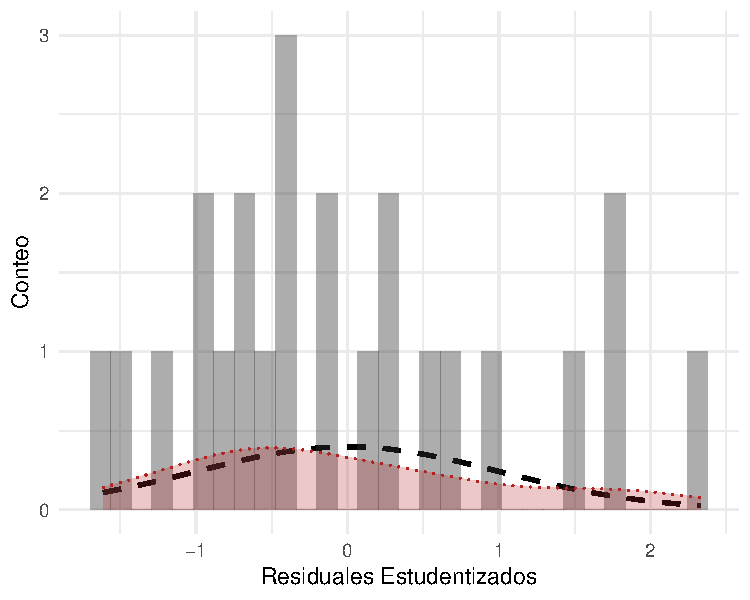
\includegraphics{diagnosticorrpp_files/figure-latex/gráfica para distribución de residuales-1.pdf}
\caption{Histograma de distribución de los residuales}
\end{figure}

\begin{figure}
\centering
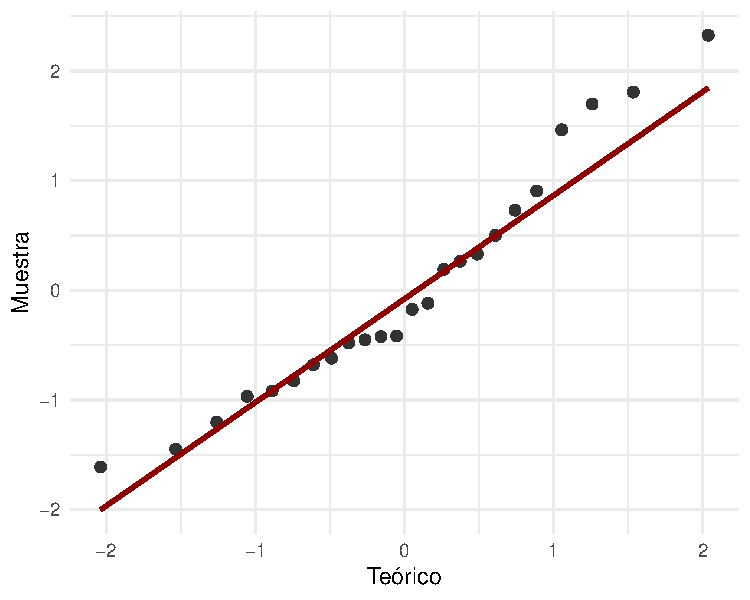
\includegraphics{diagnosticorrpp_files/figure-latex/qqplot para distribuciones de residuales-1.pdf}
\caption{Q-Q Plot: residuales estudentizados}
\end{figure}

Seguidamente se evaluó la premisa:
\(\epsilon_i \approx N(\mu =0, var=\sigma^2)\), incialmente a través de
un gráfico de distribución de los residuales estudentizados (figura 6 y
7 respectivamente). En la figura 6 se muestra que a distribución de los
residuales estudentizados (linea y sombreado rojo) es levemente
asimétrica con una desviación hacia la derecha con respecto a una curva
de normalidad (linea negra entrecortada) que cumple con los parametros
de la premisa a validar. Por su parte, la figura 7 muestra que las
observaciones finales se alejan de la linea central (roja) sugiriendo
que estas observaciones son las que pueden estár moviendo la
distribución.

\begin{longtable}[]{@{}cc@{}}
\caption{Test de shapiro-wilk (w) para los residuales}\tabularnewline
\toprule
\begin{minipage}[b]{0.12\columnwidth}\centering
\(W\)\strut
\end{minipage} & \begin{minipage}[b]{0.16\columnwidth}\centering
\(p-value\)\strut
\end{minipage}\tabularnewline
\midrule
\endfirsthead
\toprule
\begin{minipage}[b]{0.12\columnwidth}\centering
\(W\)\strut
\end{minipage} & \begin{minipage}[b]{0.16\columnwidth}\centering
\(p-value\)\strut
\end{minipage}\tabularnewline
\midrule
\endhead
\begin{minipage}[t]{0.12\columnwidth}\centering
0.9505\strut
\end{minipage} & \begin{minipage}[t]{0.16\columnwidth}\centering
0.2772\strut
\end{minipage}\tabularnewline
\bottomrule
\end{longtable}

Para comprar la normalidad de los residuales estudentizados se decidió
comprobar a través de un test de Shapiro-Wilk, el cual permite constatar
la normalidad del conjunto de observaciones, y se formula de la
siguiente manera (donde \(N\) indica una distribución normal:

\[
H_o: el\ conjunto \ de\ datos = N
\]

\[
H_1: el\ conjunto \ de\ datos \neq N 
\] El resultado obtenido de este estadístico es presentado en la tabla
10, mostrando que su resultado No tiene significancia
(\(p - value < 0.05\)). Por esta razón, no es posible rechazar la
hipotesis nula, así que se puede aseverar que los residuales
estudentizados siguen una distribución normal (\(N\)), por lo cual se
valida \(\epsilon_i \approx N(\mu =0, var=\sigma^2)\).

df 5

\begin{longtable}[]{@{}ccc@{}}
\caption{Test de Breusch-Pagan (BP) para los residuales}\tabularnewline
\toprule
\begin{minipage}[b]{0.10\columnwidth}\centering
\(BP\)\strut
\end{minipage} & \begin{minipage}[b]{0.23\columnwidth}\centering
Grados\_libertad\strut
\end{minipage} & \begin{minipage}[b]{0.15\columnwidth}\centering
\(p-value\)\strut
\end{minipage}\tabularnewline
\midrule
\endfirsthead
\toprule
\begin{minipage}[b]{0.10\columnwidth}\centering
\(BP\)\strut
\end{minipage} & \begin{minipage}[b]{0.23\columnwidth}\centering
Grados\_libertad\strut
\end{minipage} & \begin{minipage}[b]{0.15\columnwidth}\centering
\(p-value\)\strut
\end{minipage}\tabularnewline
\midrule
\endhead
\begin{minipage}[t]{0.10\columnwidth}\centering
3.176\strut
\end{minipage} & \begin{minipage}[t]{0.23\columnwidth}\centering
5\strut
\end{minipage} & \begin{minipage}[t]{0.15\columnwidth}\centering
0.6728\strut
\end{minipage}\tabularnewline
\bottomrule
\end{longtable}

Para evaluar si existe homocedasticidad (\(var(\epsilon_i) = \sigma^2\))
en los residuales estandarizados, se recurrió a realizar un test de
Breusch-Pagan, el cual establece si la varianza estimada dependen de las
observaciones de manera independiente, se supone homocedasticidad en
cuando no hay esta dependecia, y heterocedasticidad en cuanto si existe
esta dependencia. Esto se establece de la siguiente forma:

\[
H_o: hay \ homocedasticidad
\]

\[
H_1: hay \ heterocedasticidad 
\] El resultado obtenido del test de Breusch-Pagan es presentado en la
tabla 11, mostrando que su resultado No tiene significancia
(\(p - value < 0.05\)). Por esta razón, no es posible rechazar la
hipotesis nula, así que se puede aseverar que los hay homocedasticidad,
es decir la varianza no depende de las observaciones independientes sino
deel modelo en su totalidad, por lo cual se valida
(\(var(\epsilon_i) = \sigma^2\)).

\begin{longtable}[]{@{}cc@{}}
\caption{Test de Durbin--Watson (DW) para los residuales}\tabularnewline
\toprule
\begin{minipage}[b]{0.10\columnwidth}\centering
\(DW\)\strut
\end{minipage} & \begin{minipage}[b]{0.16\columnwidth}\centering
\(p-value\)\strut
\end{minipage}\tabularnewline
\midrule
\endfirsthead
\toprule
\begin{minipage}[b]{0.10\columnwidth}\centering
\(DW\)\strut
\end{minipage} & \begin{minipage}[b]{0.16\columnwidth}\centering
\(p-value\)\strut
\end{minipage}\tabularnewline
\midrule
\endhead
\begin{minipage}[t]{0.10\columnwidth}\centering
2.097\strut
\end{minipage} & \begin{minipage}[t]{0.16\columnwidth}\centering
0.5757\strut
\end{minipage}\tabularnewline
\bottomrule
\end{longtable}

Finalmente, Para evaluar si existe autocorrelación
\(corr(\epsilon_i, \epsilon_j) = 0\) entre los residuales
estandarizados, se recurrió a realizar un test de Durbin--Watson, el
cual establece que si la autocorrelación designada con el simbolo
\(\rho\) es igual a 0 (\(\rho = 0\)) entonces las observaciones no están
autocorrelacionados, en cambio si existe autocorrelación
(\(\rho \neq 0\)) entonces algunas de las observaciones están
correlacionadas . Esto se establece de la siguiente forma:

\[
H_o: \rho = 0
\]

\[
H_1: \rho \neq 0 
\] La tabla 12 muestra los resultados del test de Durbin--Watson. Este
muestra que No existe significancia (\(p - value < 0.05\)). Por esta
razón, no es posible rechazar la hipotesis nula, así que se puede
aseverar que los residuales estudentizados no se encuentran
correlacionados entre ellos.

\hypertarget{pregunta-7-realice-un-anuxe1lisis-de-diagnuxf3stico-e-identifuxedue-si-es-que-existen-observaciones-con-alto-leverage-incluyentes-y-extremas-en-la-respuesta.}{%
\subsubsection{Pregunta \#7: Realice un análisis de diagnóstico e
identifíue (si es que existen) observaciones con alto leverage,
incluyentes y extremas en la
respuesta.}\label{pregunta-7-realice-un-anuxe1lisis-de-diagnuxf3stico-e-identifuxedue-si-es-que-existen-observaciones-con-alto-leverage-incluyentes-y-extremas-en-la-respuesta.}}

La figura 8, 9 y 10 corresponden al análisis de los residuales
estudentizados para evaluar el efecto de cada una de las observaciones
en el mejor modelo de regresión encontrado por los métodos y
estadísticos previamente descritos.

\begin{figure}
\centering
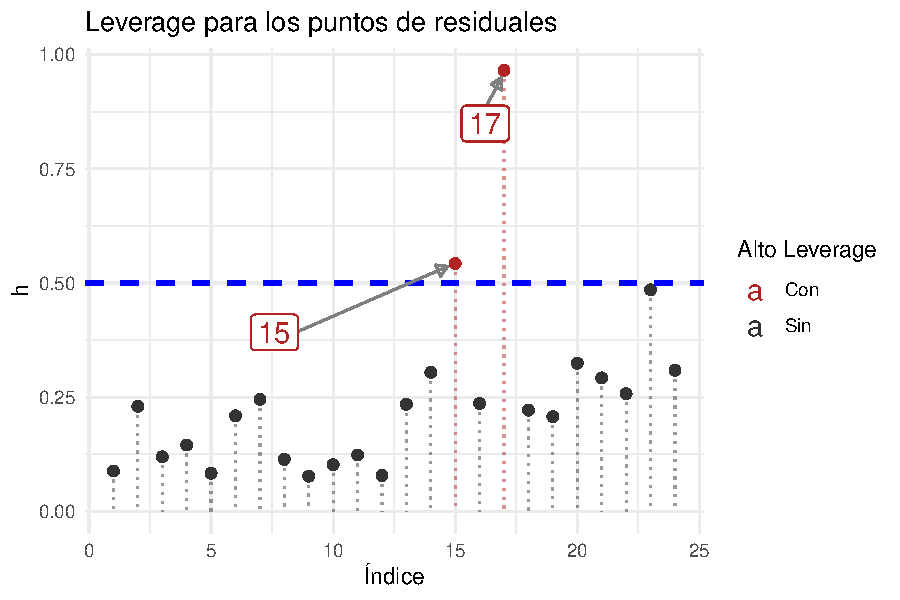
\includegraphics{diagnosticorrpp_files/figure-latex/residuals LEVERAGE para bestmodel-1.pdf}
\caption{Evaluación de altos \emph{leverage} para el mejor modelo}
\end{figure}

La figura 8, en el eje \(x\) muesta el número de la observación o
(índice) y la \(y\) los valores correspondientes la diagonal de la
matriz H obtenida de los residuales estudentizados y predichos. la linea
azul traza el punto donde los valores de la diagonal en H son dos veces
la media de estos valores. Como se puede evidenciar la observación
número 15 y 17 son superiores a dos veces la media de los valores en H,
de manera que se consideran valores con alto \emph{leverage} (o
apalancamiento), es decir que estas observaciones pueden afectar la
regresión.

\begin{figure}
\centering
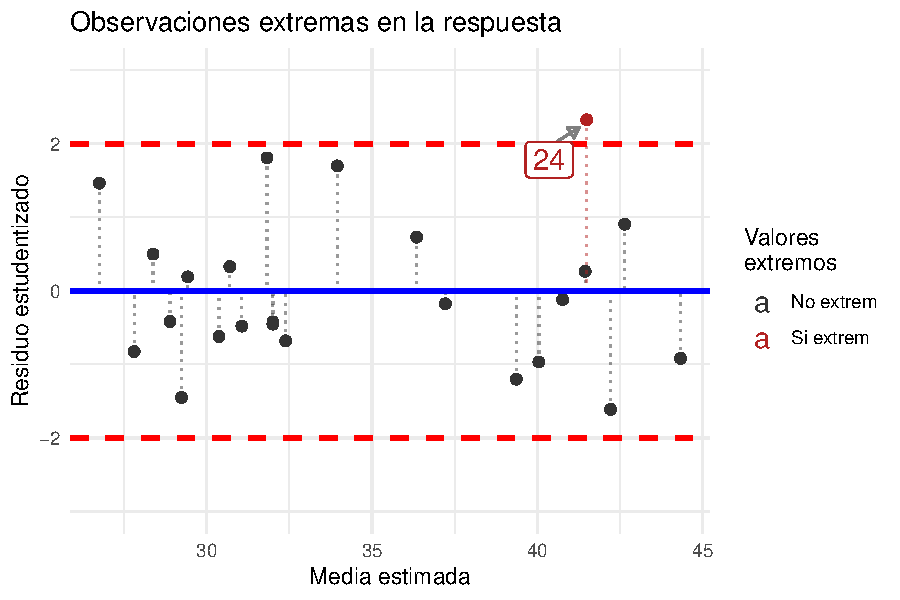
\includegraphics{diagnosticorrpp_files/figure-latex/observaciones EXTREMAS para bestmodel-1.pdf}
\caption{Evaluación de observaciones extremas para el mejor modelo}
\end{figure}

La figura 9, en el eje \(x\) muestra a la media estimada de los
residuales estimados por el modelo, y \(y\) los valores correspondientes
a los valores que toman los residuales estudentizados. la linea azul
traza el punto 0 y las lineas rojas entre cortadas, las desviaciones
estandar de los residuales estudentizados (2 y -2 sd). Como se puede
evidenciar la observación número 24 esta fuera de dos deviaciones
estandar por lo cual de considera una observación extrema y se debe
evaluar si es influyente.

\begin{figure}
\centering
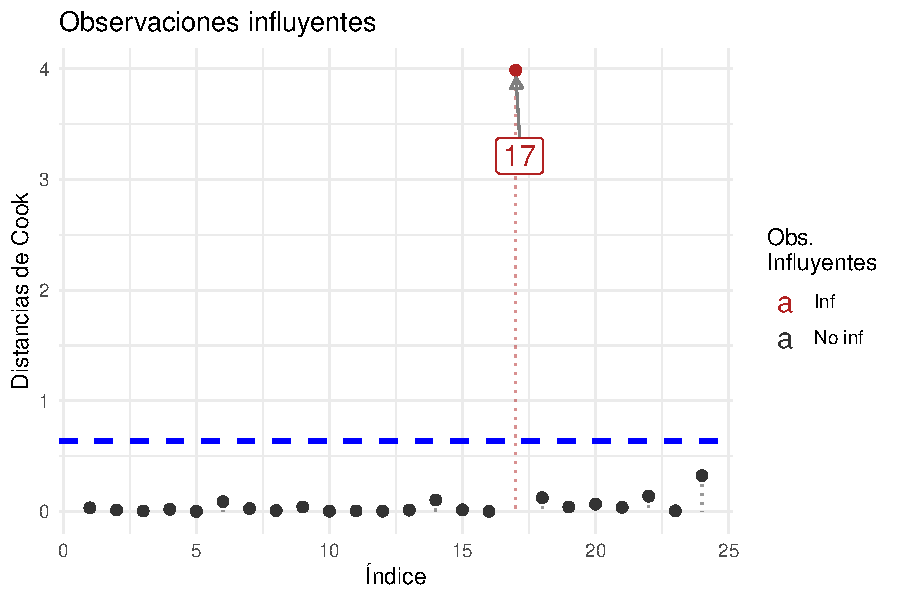
\includegraphics{diagnosticorrpp_files/figure-latex/observaciones influyentes para bestmodel-1.pdf}
\caption{Evaluación de observaciones influyentes para el mejor modelo}
\end{figure}

Finalmente la figura 10, en el eje \(x\) muesta el número de la
observación o (índice), y \(y\) los valores correspondientes a las
distancias de Cook, que evaluan la influencia de las observaciones en el
modelo. la linea azul traza el valor que corresponde la desviación 3
veces de promedio de los residuales estudentizados. Como se puede
evidenciar la observación número 17 es la observación más influyente en
el modelo además que ejerce \emph{leverage} de manera que sería
conveniente sustraer esta observación y evaluar nuevamente su efecto en
el modelo.

\hypertarget{evaluaciuxf3n-de-mejor-modelo-sin-la-observaciuxf3n-influyente}{%
\subsection{Evaluación de mejor modelo sin la observación
influyente}\label{evaluaciuxf3n-de-mejor-modelo-sin-la-observaciuxf3n-influyente}}

\hypertarget{anuxe1lisis-de-estimadores-y-t-values-mejor-modelo-excluyendo-observaciuxf3n-influyente-17}{%
\subsubsection{\texorpdfstring{Análisis de estimadores y \(t-values\)
mejor modelo excluyendo observación influyente
\#17}{Análisis de estimadores y t-values mejor modelo excluyendo observación influyente \#17}}\label{anuxe1lisis-de-estimadores-y-t-values-mejor-modelo-excluyendo-observaciuxf3n-influyente-17}}

La tabla 12 presenta las estimaciones del ``mejor modelo'' excluyendo
observación influyente y sus \(t-values\). Allí se evidencia un estimado
del intercepto (\texttt{precioventa}) con valor positivo \(> 0\) (20.2);
de manera que de estos resultados se puede deducir que algunos
estimadores de las variables regresoras, pueden afectar el resultado de
la variable respuesta. Al verificar los \(t-values\) se observa que solo
son significativas nuevamente \texttt{num\_banos} al igual que el modelo
original (\(p - value < 0.05\)). Las demás variables regresoras
utilizadas en este modelo no son significativas
(\(p - value \geq 0.05\)), así pues, no es posible establecer que puedan
tener efecto alguno sobre la variable respuesta. De acá se se puede
inferir que un incremento en una unidad del numero de baños se puede
incrementar 6.08/1000 dolares el precio de venta de la propiedad siempre
que las otras variables no cambien.

\begin{longtable}[]{@{}ccccc@{}}
\caption{Estimadores, \(t-values\) y significancia para el mejor modelo
sugerido por AIC, Cp, y \(r^2_{adj}\)}\tabularnewline
\toprule
\begin{minipage}[b]{0.26\columnwidth}\centering
~\strut
\end{minipage} & \begin{minipage}[b]{0.13\columnwidth}\centering
Estimado\strut
\end{minipage} & \begin{minipage}[b]{0.16\columnwidth}\centering
ErrorStand\strut
\end{minipage} & \begin{minipage}[b]{0.14\columnwidth}\centering
\(t-value\)\strut
\end{minipage} & \begin{minipage}[b]{0.14\columnwidth}\centering
\(p-value\)\strut
\end{minipage}\tabularnewline
\midrule
\endfirsthead
\toprule
\begin{minipage}[b]{0.26\columnwidth}\centering
~\strut
\end{minipage} & \begin{minipage}[b]{0.13\columnwidth}\centering
Estimado\strut
\end{minipage} & \begin{minipage}[b]{0.16\columnwidth}\centering
ErrorStand\strut
\end{minipage} & \begin{minipage}[b]{0.14\columnwidth}\centering
\(t-value\)\strut
\end{minipage} & \begin{minipage}[b]{0.14\columnwidth}\centering
\(p-value\)\strut
\end{minipage}\tabularnewline
\midrule
\endhead
\begin{minipage}[t]{0.26\columnwidth}\centering
\textbf{(Intercept)}\strut
\end{minipage} & \begin{minipage}[t]{0.13\columnwidth}\centering
20.2\strut
\end{minipage} & \begin{minipage}[t]{0.16\columnwidth}\centering
3.82\strut
\end{minipage} & \begin{minipage}[t]{0.14\columnwidth}\centering
5.3\strut
\end{minipage} & \begin{minipage}[t]{0.14\columnwidth}\centering
5.92e-05\strut
\end{minipage}\tabularnewline
\begin{minipage}[t]{0.26\columnwidth}\centering
\textbf{impuestos}\strut
\end{minipage} & \begin{minipage}[t]{0.13\columnwidth}\centering
1.07\strut
\end{minipage} & \begin{minipage}[t]{0.16\columnwidth}\centering
0.74\strut
\end{minipage} & \begin{minipage}[t]{0.14\columnwidth}\centering
1.45\strut
\end{minipage} & \begin{minipage}[t]{0.14\columnwidth}\centering
0.165\strut
\end{minipage}\tabularnewline
\begin{minipage}[t]{0.26\columnwidth}\centering
\textbf{num\_banos}\strut
\end{minipage} & \begin{minipage}[t]{0.13\columnwidth}\centering
6.08\strut
\end{minipage} & \begin{minipage}[t]{0.16\columnwidth}\centering
1.87\strut
\end{minipage} & \begin{minipage}[t]{0.14\columnwidth}\centering
3.25\strut
\end{minipage} & \begin{minipage}[t]{0.14\columnwidth}\centering
0.00476\strut
\end{minipage}\tabularnewline
\begin{minipage}[t]{0.26\columnwidth}\centering
\textbf{num\_puestos\_gar}\strut
\end{minipage} & \begin{minipage}[t]{0.13\columnwidth}\centering
1.49\strut
\end{minipage} & \begin{minipage}[t]{0.16\columnwidth}\centering
1.03\strut
\end{minipage} & \begin{minipage}[t]{0.14\columnwidth}\centering
1.45\strut
\end{minipage} & \begin{minipage}[t]{0.14\columnwidth}\centering
0.166\strut
\end{minipage}\tabularnewline
\begin{minipage}[t]{0.26\columnwidth}\centering
\textbf{edad\_hogar}\strut
\end{minipage} & \begin{minipage}[t]{0.13\columnwidth}\centering
-0.0926\strut
\end{minipage} & \begin{minipage}[t]{0.16\columnwidth}\centering
0.0484\strut
\end{minipage} & \begin{minipage}[t]{0.14\columnwidth}\centering
-1.91\strut
\end{minipage} & \begin{minipage}[t]{0.14\columnwidth}\centering
0.0729\strut
\end{minipage}\tabularnewline
\begin{minipage}[t]{0.26\columnwidth}\centering
\textbf{cant\_chimen}\strut
\end{minipage} & \begin{minipage}[t]{0.13\columnwidth}\centering
2.62\strut
\end{minipage} & \begin{minipage}[t]{0.16\columnwidth}\centering
1.29\strut
\end{minipage} & \begin{minipage}[t]{0.14\columnwidth}\centering
2.03\strut
\end{minipage} & \begin{minipage}[t]{0.14\columnwidth}\centering
0.0578\strut
\end{minipage}\tabularnewline
\bottomrule
\end{longtable}

La tabla 13 muestra los resultados para el estadístico \(F\) de Fisher
con 17 grados de libertad, donde el \(p-value\) demuestra significancia
estadística (\(p - value < 0.05\)), con lo que se rechaza la hipotesis
nula. De tal forma, se puede inferir que almenos una de la variables
regresoras (\(\beta_i\)) son diferentes de 0.

La tabla 14, muestra los resultados de los \(R^2\) y \(R_{adj}^2\) para
el ``modelo de regresión original''mejor modelo" sin observación
influyente. De esto se puede inferir que aproximadamente el 81\% de la
variabilidad de la variable respuesta (\texttt{precioventa}) puede ser
explicado por las variables regresoras del ``mejor modelo'' y la
variabilidad restante puede ser consecuencia a otras variables no
tenidas encuenta en el modelo o por azar.

\begin{longtable}[]{@{}ccc@{}}
\caption{Estadistico \(F\) de Fisher: significancia del mejor
modelo}\tabularnewline
\toprule
\begin{minipage}[b]{0.24\columnwidth}\centering
\(F_{stat}\)\strut
\end{minipage} & \begin{minipage}[b]{0.23\columnwidth}\centering
Grados\_libertad\strut
\end{minipage} & \begin{minipage}[b]{0.15\columnwidth}\centering
\(p-value\)\strut
\end{minipage}\tabularnewline
\midrule
\endfirsthead
\toprule
\begin{minipage}[b]{0.24\columnwidth}\centering
\(F_{stat}\)\strut
\end{minipage} & \begin{minipage}[b]{0.23\columnwidth}\centering
Grados\_libertad\strut
\end{minipage} & \begin{minipage}[b]{0.15\columnwidth}\centering
\(p-value\)\strut
\end{minipage}\tabularnewline
\midrule
\endhead
\begin{minipage}[t]{0.24\columnwidth}\centering
20.2777398941543\strut
\end{minipage} & \begin{minipage}[t]{0.23\columnwidth}\centering
17\strut
\end{minipage} & \begin{minipage}[t]{0.15\columnwidth}\centering
1.275e-06\strut
\end{minipage}\tabularnewline
\bottomrule
\end{longtable}

\begin{longtable}[]{@{}cc@{}}
\caption{\(R^2\) y \(R_{adj}^2\) para el modelo}\tabularnewline
\toprule
\endhead
\begin{minipage}[t]{0.10\columnwidth}\centering
0.856\strut
\end{minipage} & \begin{minipage}[t]{0.10\columnwidth}\centering
0.814\strut
\end{minipage}\tabularnewline
\bottomrule
\end{longtable}

\hypertarget{anuxe1lisis-de-residuales-del-mejor-modelo-excluyendo-observaciuxf3n-influyente-17}{%
\subsubsection{Análisis de residuales del mejor modelo excluyendo
observación influyente
\#17}\label{anuxe1lisis-de-residuales-del-mejor-modelo-excluyendo-observaciuxf3n-influyente-17}}

La figura 11, 12 y 13 corresponden al análisis de los residuales
estudentizados para evaluar el efecto de cada una de las observaciones
en el mejor modelo excluyendo la observación influyente del ``mejor
modelo''. A partir de esto es de notar que la observación 23 aparece
como extrema e influyente pero sin alto \emph{leverage}. En su lugar,
presentan alto \emph{leverage} la observación 15 y 22. De estas la
observación 15 previamente había presentado alto \emph{leverage} en el
``mejor modelo'', sin embargo, aparece en este modelo como no
influyente.

\begin{figure}
\centering
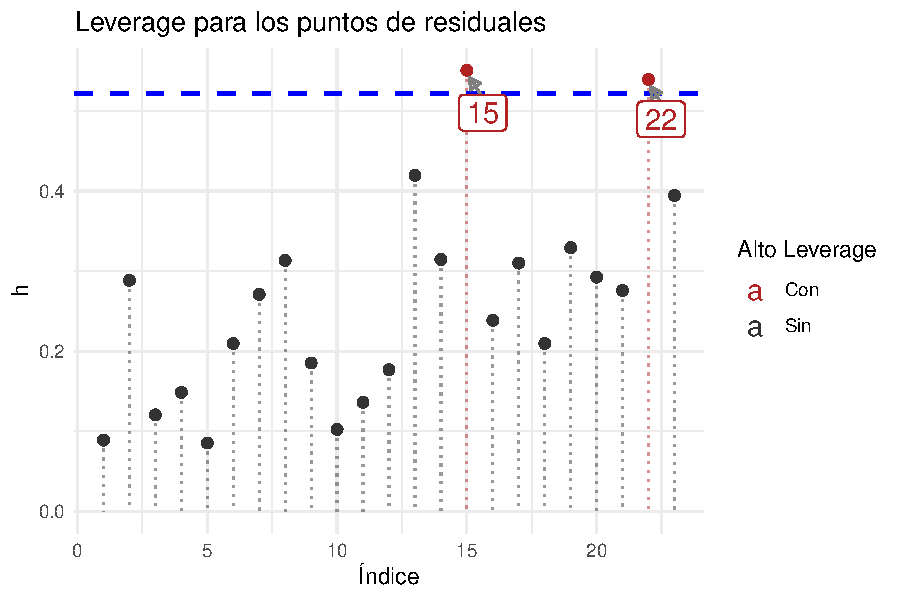
\includegraphics{diagnosticorrpp_files/figure-latex/residuals LEVERAGE para bestmodel sin 17-1.pdf}
\caption{Evaluación de altos \emph{leverage} para el mejor modelo sin
observación influyente}
\end{figure}

\begin{figure}
\centering
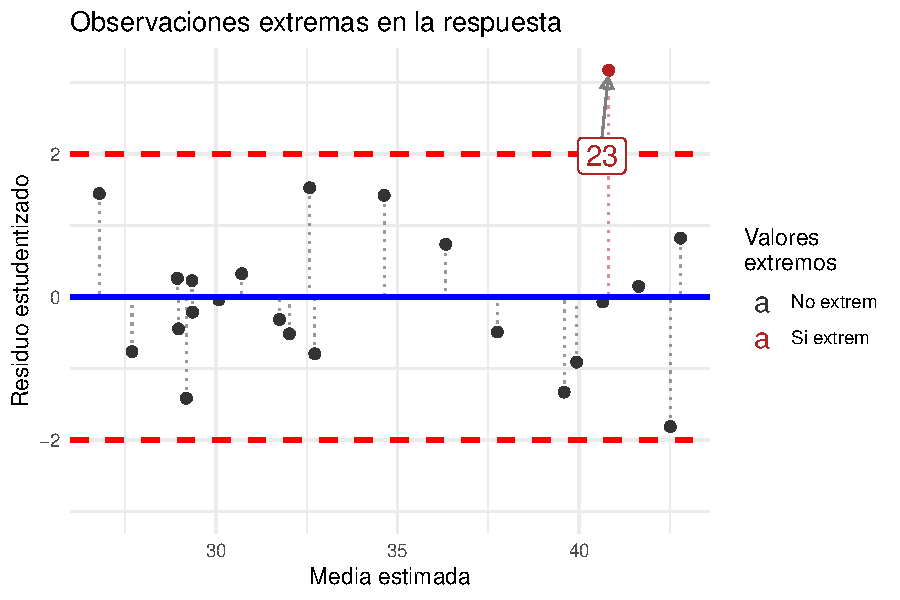
\includegraphics{diagnosticorrpp_files/figure-latex/observaciones EXTREMAS para bestmodel sin 17-1.pdf}
\caption{Evaluación de observaciones extremas para el mejor modelo sin
observación influyente}
\end{figure}

\begin{figure}
\centering
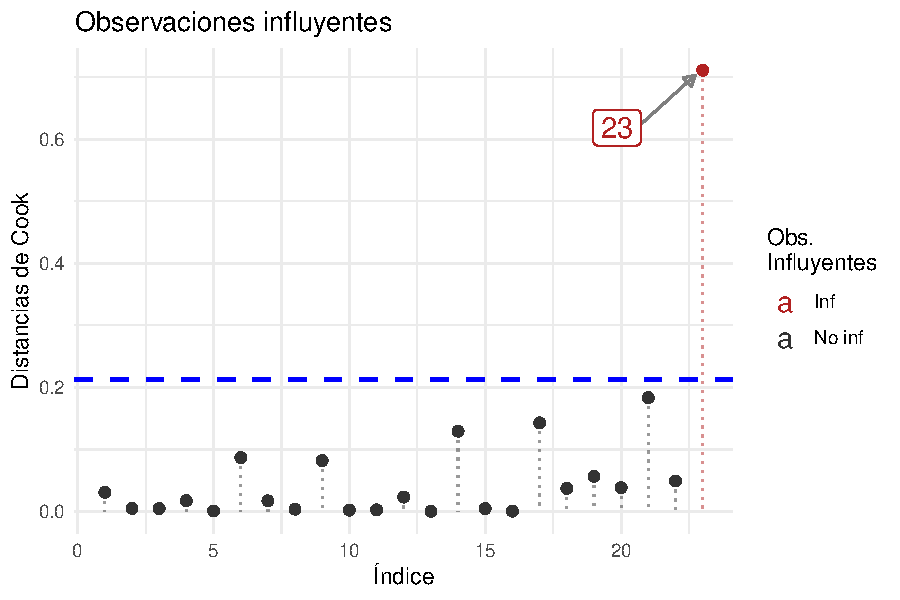
\includegraphics{diagnosticorrpp_files/figure-latex/observaciones influyentes para bestmodel sin 17-1.pdf}
\caption{Evaluación de observaciones influyentes para el mejor modelo
sin observación influyente}
\end{figure}

\hypertarget{anexo-mejor-modelo-por-bic}{%
\section{Anexo (mejor modelo por
BIC)}\label{anexo-mejor-modelo-por-bic}}

\hypertarget{se-realizuxf3-mejor-modelo-por-bic-con-dos-variables-regresoras-impuestos-y-num_banos-con-todas-las-observaciones.}{%
\subsection{\texorpdfstring{Se realizó mejor modelo por \(BIC\) con dos
variables regresoras \texttt{impuestos} y \texttt{num\_banos}, con todas
las
observaciones.}{Se realizó mejor modelo por BIC con dos variables regresoras impuestos y num\_banos, con todas las observaciones.}}\label{se-realizuxf3-mejor-modelo-por-bic-con-dos-variables-regresoras-impuestos-y-num_banos-con-todas-las-observaciones.}}

\hypertarget{estimadores-y-t-values-para-el-mejor-modelo-por-bic}{%
\subsubsection{\texorpdfstring{EStimadores y \(t-values\) para el mejor
modelo por
BIC}{EStimadores y t-values para el mejor modelo por BIC}}\label{estimadores-y-t-values-para-el-mejor-modelo-por-bic}}

La tabla 15 presenta las estimaciones del ``mejor modelo por BIC'' y sus
\(t-values\). Allí se evidencia un estimado del intercepto
(\texttt{precioventa}) con valor positivo \(> 0\) (13.1); de manera que
de estos resultados se puede deducir que algunos estimadores de las
variables regresoras, pueden afectar el resultado de la variable
respuesta. Al verificar los \(t-values\) se observa que solo es
significativa la variable \texttt{impuestos}. En este caso la variable
\texttt{num\_banos}que había sido significativa en los otros dos modelos
es no son significativas (\(p - value \geq 0.05\)) en este. Por esto, se
puede establecer que \texttt{impuestos} puedan tener efecto alguno sobre
la variable respuesta. De acá se se puede inferir que un incremento en
una unidad de impuestos se puede incrementar 2.71/1000 dolares el precio
de venta de la propiedad siempre que las otras variables no cambien.

\begin{longtable}[]{@{}ccccc@{}}
\caption{Estimadores, \(t-values\) y significancia para el mejor modelo
sugerido por BIC\$}\tabularnewline
\toprule
\begin{minipage}[b]{0.21\columnwidth}\centering
~\strut
\end{minipage} & \begin{minipage}[b]{0.13\columnwidth}\centering
Estimado\strut
\end{minipage} & \begin{minipage}[b]{0.16\columnwidth}\centering
ErrorStand\strut
\end{minipage} & \begin{minipage}[b]{0.14\columnwidth}\centering
\(t-value\)\strut
\end{minipage} & \begin{minipage}[b]{0.14\columnwidth}\centering
\(p-value\)\strut
\end{minipage}\tabularnewline
\midrule
\endfirsthead
\toprule
\begin{minipage}[b]{0.21\columnwidth}\centering
~\strut
\end{minipage} & \begin{minipage}[b]{0.13\columnwidth}\centering
Estimado\strut
\end{minipage} & \begin{minipage}[b]{0.16\columnwidth}\centering
ErrorStand\strut
\end{minipage} & \begin{minipage}[b]{0.14\columnwidth}\centering
\(t-value\)\strut
\end{minipage} & \begin{minipage}[b]{0.14\columnwidth}\centering
\(p-value\)\strut
\end{minipage}\tabularnewline
\midrule
\endhead
\begin{minipage}[t]{0.21\columnwidth}\centering
\textbf{(Intercept)}\strut
\end{minipage} & \begin{minipage}[t]{0.13\columnwidth}\centering
13.1\strut
\end{minipage} & \begin{minipage}[t]{0.16\columnwidth}\centering
2.43\strut
\end{minipage} & \begin{minipage}[t]{0.14\columnwidth}\centering
5.41\strut
\end{minipage} & \begin{minipage}[t]{0.14\columnwidth}\centering
2.31e-05\strut
\end{minipage}\tabularnewline
\begin{minipage}[t]{0.21\columnwidth}\centering
\textbf{impuestos}\strut
\end{minipage} & \begin{minipage}[t]{0.13\columnwidth}\centering
2.71\strut
\end{minipage} & \begin{minipage}[t]{0.16\columnwidth}\centering
0.485\strut
\end{minipage} & \begin{minipage}[t]{0.14\columnwidth}\centering
5.6\strut
\end{minipage} & \begin{minipage}[t]{0.14\columnwidth}\centering
1.49e-05\strut
\end{minipage}\tabularnewline
\begin{minipage}[t]{0.21\columnwidth}\centering
\textbf{num\_banos}\strut
\end{minipage} & \begin{minipage}[t]{0.13\columnwidth}\centering
3.08\strut
\end{minipage} & \begin{minipage}[t]{0.16\columnwidth}\centering
1.59\strut
\end{minipage} & \begin{minipage}[t]{0.14\columnwidth}\centering
1.93\strut
\end{minipage} & \begin{minipage}[t]{0.14\columnwidth}\centering
0.0666\strut
\end{minipage}\tabularnewline
\bottomrule
\end{longtable}

La tabla 16 muestra los resultados para el estadístico \(F\) de Fisher
con 21 grados de libertad, donde el \(p-value\) demuestra significancia
estadística (\(p - value < 0.05\)), con lo que se rechaza la hipotesis
nula. De tal forma, se puede inferir que almenos una de la variables
regresoras (\(\beta_i\)) son diferentes de 0.

La tabla 17, muestra los resultados de los \(R^2\) y \(R_{adj}^2\) para
el ``modelo de regresión original''mejor modelo por BIC``. De esto se
puede inferir que aproximadamente el 78\% de la variabilidad de la
variable respuesta (\texttt{precioventa}) puede ser explicado por las
variables regresoras del''mejor modelo por BIC" y la variabilidad
restante puede ser consecuencia a otras variables no tenidas encuenta en
el modelo o por azar. Esto es esperado por que el resultado del
estadístico \(R_{adj}^2\) para selección de modelo daba como mejor el
seleccionado como ``mejor modelo'' o sea el modelo de 5 variables.

\begin{longtable}[]{@{}ccc@{}}
\caption{Estadistico \(F\) de Fisher: significancia del mejor modelo por
\(BIC\)}\tabularnewline
\toprule
\begin{minipage}[b]{0.24\columnwidth}\centering
\(F_{stat}\)\strut
\end{minipage} & \begin{minipage}[b]{0.23\columnwidth}\centering
Grados\_libertad\strut
\end{minipage} & \begin{minipage}[b]{0.15\columnwidth}\centering
\(p-value\)\strut
\end{minipage}\tabularnewline
\midrule
\endfirsthead
\toprule
\begin{minipage}[b]{0.24\columnwidth}\centering
\(F_{stat}\)\strut
\end{minipage} & \begin{minipage}[b]{0.23\columnwidth}\centering
Grados\_libertad\strut
\end{minipage} & \begin{minipage}[b]{0.15\columnwidth}\centering
\(p-value\)\strut
\end{minipage}\tabularnewline
\midrule
\endhead
\begin{minipage}[t]{0.24\columnwidth}\centering
42.6719279014923\strut
\end{minipage} & \begin{minipage}[t]{0.23\columnwidth}\centering
21\strut
\end{minipage} & \begin{minipage}[t]{0.15\columnwidth}\centering
4.007e-08\strut
\end{minipage}\tabularnewline
\bottomrule
\end{longtable}

\begin{longtable}[]{@{}cc@{}}
\caption{\(R^2\) y \(R_{adj}^2\) para el mejor modelo por
\(BIC\)}\tabularnewline
\toprule
\begin{minipage}[b]{0.10\columnwidth}\centering
\(R^2\)\strut
\end{minipage} & \begin{minipage}[b]{0.18\columnwidth}\centering
\(R_{adj}^2\)\strut
\end{minipage}\tabularnewline
\midrule
\endfirsthead
\toprule
\begin{minipage}[b]{0.10\columnwidth}\centering
\(R^2\)\strut
\end{minipage} & \begin{minipage}[b]{0.18\columnwidth}\centering
\(R_{adj}^2\)\strut
\end{minipage}\tabularnewline
\midrule
\endhead
\begin{minipage}[t]{0.10\columnwidth}\centering
0.803\strut
\end{minipage} & \begin{minipage}[t]{0.18\columnwidth}\centering
0.784\strut
\end{minipage}\tabularnewline
\bottomrule
\end{longtable}

\hypertarget{validaciuxf3n-del-mejor-modelo-bic}{%
\subsubsection{\texorpdfstring{Validación del mejor modelo
\(BIC\)}{Validación del mejor modelo BIC}}\label{validaciuxf3n-del-mejor-modelo-bic}}

Para determinar la validez del mejor modelo obtenido por \(BIC\) se
evaluaron los mismos parametros que el modelo original.

Inicialmente se evaluó la premisa \(\epsilon_i = 0\). La figura 14,
muestra que hay cierta variabilidad entre las relaciones, dadas por
algunas observaciones extremas que se alejan de 0 al igual que el
``mejor modelo'' obtenido por otros estadísticos.

\begin{figure}
\centering
\includegraphics{diagnosticorrpp_files/figure-latex/distribución de los resdiuos por BIC-1.pdf}
\caption{Distribución de los residuales estudentizados del modelo por
\(BIC\)}
\end{figure}

A continuación se evaluó la premisa:
\(\epsilon_i \approx N(\mu =0, var=\sigma^2)\), incialmente a través de
un gráfico de distribución de los residuales estudentizados (figura 15),
este muestra que a distribución de los residuales estudentizados para
este modelo (linea y sombreado rojo) continua levemente asimétrica con
una desviación hacia la derecha con respecto a una curva de normalidad
(linea negra entrecortada) que cumple con los parametros de la premisa a
validar, caso similar a lo ocurrido en el ``mejor modelo'' de 5
variables.

\begin{figure}
\centering
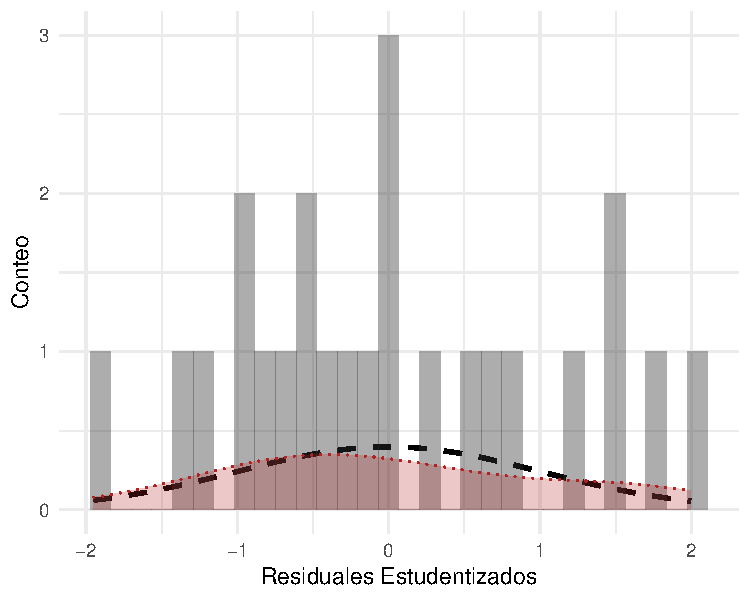
\includegraphics{diagnosticorrpp_files/figure-latex/gráfica para distribución de residuales por BIC-1.pdf}
\caption{Histograma de distribución de los residuales del modelo por
\(BIC\)}
\end{figure}

\begin{longtable}[]{@{}cc@{}}
\caption{Test de shapiro-wilk (w) para los residuales}\tabularnewline
\toprule
\begin{minipage}[b]{0.12\columnwidth}\centering
\(W\)\strut
\end{minipage} & \begin{minipage}[b]{0.16\columnwidth}\centering
\(p-value\)\strut
\end{minipage}\tabularnewline
\midrule
\endfirsthead
\toprule
\begin{minipage}[b]{0.12\columnwidth}\centering
\(W\)\strut
\end{minipage} & \begin{minipage}[b]{0.16\columnwidth}\centering
\(p-value\)\strut
\end{minipage}\tabularnewline
\midrule
\endhead
\begin{minipage}[t]{0.12\columnwidth}\centering
0.9709\strut
\end{minipage} & \begin{minipage}[t]{0.16\columnwidth}\centering
0.6897\strut
\end{minipage}\tabularnewline
\bottomrule
\end{longtable}

La tabla 18, muestra el resultado del test de shapiro-Wilk cuyo
resultado No tiene significancia (\(p - value < 0.05\)). Por esta razón,
no es posible rechazar la hipotesis nula, así que se puede aseverar que
los residuales estudentizados para este modelo obtenido por \(BIC\)
siguen una distribución normal (\(N\)), por lo cual se valida
\(\epsilon_i \approx N(\mu =0, var=\sigma^2)\).

\begin{longtable}[]{@{}ccc@{}}
\caption{Test de Breusch-Pagan (BP) para los residuales}\tabularnewline
\toprule
\begin{minipage}[b]{0.11\columnwidth}\centering
\(BP\)\strut
\end{minipage} & \begin{minipage}[b]{0.23\columnwidth}\centering
Grados\_libertad\strut
\end{minipage} & \begin{minipage}[b]{0.15\columnwidth}\centering
\(p-value\)\strut
\end{minipage}\tabularnewline
\midrule
\endfirsthead
\toprule
\begin{minipage}[b]{0.11\columnwidth}\centering
\(BP\)\strut
\end{minipage} & \begin{minipage}[b]{0.23\columnwidth}\centering
Grados\_libertad\strut
\end{minipage} & \begin{minipage}[b]{0.15\columnwidth}\centering
\(p-value\)\strut
\end{minipage}\tabularnewline
\midrule
\endhead
\begin{minipage}[t]{0.11\columnwidth}\centering
0.3459\strut
\end{minipage} & \begin{minipage}[t]{0.23\columnwidth}\centering
2\strut
\end{minipage} & \begin{minipage}[t]{0.15\columnwidth}\centering
0.8412\strut
\end{minipage}\tabularnewline
\bottomrule
\end{longtable}

La tabla 19, muestra el resultado del test de Breusch-pagan cuyo
resultado No tiene significancia (\(p - value < 0.05\)). Por esta razón,
no es posible rechazar la hipotesis nula, así que se puede aseverar que
los hay homocedasticidad, es decir la varianza no depende de las
observaciones independientes sino deel modelo en su totalidad, por lo
cual se valida (\(var(\epsilon_i) = \sigma^2\)).

\begin{longtable}[]{@{}cc@{}}
\caption{Test de Durbin--Watson (DW) para los residuales}\tabularnewline
\toprule
\begin{minipage}[b]{0.10\columnwidth}\centering
\(DW\)\strut
\end{minipage} & \begin{minipage}[b]{0.16\columnwidth}\centering
\(p-value\)\strut
\end{minipage}\tabularnewline
\midrule
\endfirsthead
\toprule
\begin{minipage}[b]{0.10\columnwidth}\centering
\(DW\)\strut
\end{minipage} & \begin{minipage}[b]{0.16\columnwidth}\centering
\(p-value\)\strut
\end{minipage}\tabularnewline
\midrule
\endhead
\begin{minipage}[t]{0.10\columnwidth}\centering
2.161\strut
\end{minipage} & \begin{minipage}[t]{0.16\columnwidth}\centering
0.5897\strut
\end{minipage}\tabularnewline
\bottomrule
\end{longtable}

La tabla 20, muestra el resultado del test de Durbin--Watson cuyo
resultado No tiene significancia (\(p - value < 0.05\)).Por esta razón,
no es posible rechazar la hipotesis nula, así que se puede aseverar que
los residuales estudentizados para el modelo obtenido por no se
encuentran correlacionados entre ellos.

\hypertarget{anuxe1lisis-de-residuales-del-mejor-modelor-bic}{%
\subsubsection{\texorpdfstring{Análisis de residuales del mejor modelor
\(BIC\)}{Análisis de residuales del mejor modelor BIC}}\label{anuxe1lisis-de-residuales-del-mejor-modelor-bic}}

La figura 16, 17 y 18 corresponden al análisis de los residuales
estudentizados para evaluar el efecto de cada una de las observaciones
en el mejor modelo producido por el estadístico \(BIC\). A partir de
estos resultados, es importante notar que la observación 17 al igual que
el ``mejor modelo'' de 5 variables, presenta alto \emph{leverage} y es
influyente. Además llama la atención que la observación 15 previamente
había presentado alto \emph{leverage} en el ``mejor modelo'' aparece en
este modelo como una observación influyente. Además la observación \# 15
presenta alto \emph{leverage} en el ``mejor modelo'' sin observación
influyente (figura 12) de manera que es importante proponer un modelo
que excluya esta observación. Para este nuevo modelo no se obtienen
observaciones etremas.

\begin{figure}
\centering
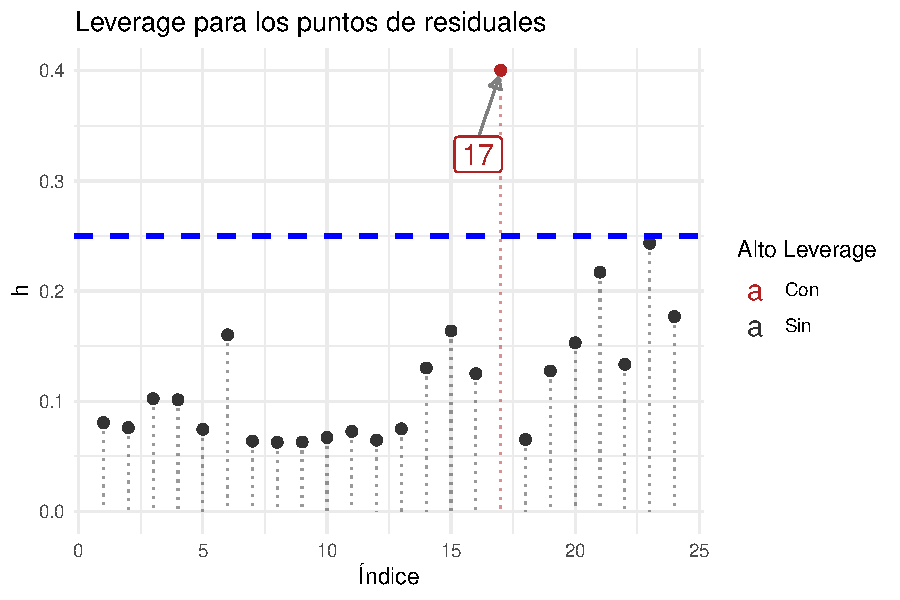
\includegraphics{diagnosticorrpp_files/figure-latex/residuals LEVERAGE para mejor modelo por BIC-1.pdf}
\caption{Evaluación de altos \emph{leverage} para el mejor modelo por
BIC}
\end{figure}

\begin{figure}
\centering
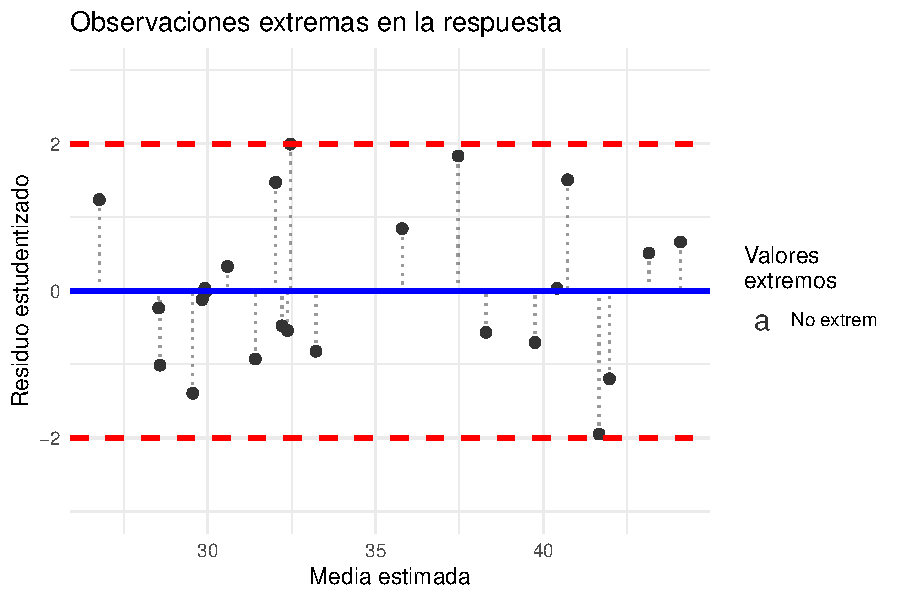
\includegraphics{diagnosticorrpp_files/figure-latex/observaciones EXTREMAS para mejor modelo por BIC-1.pdf}
\caption{Evaluación de observaciones extremas para el mejor modelo por
BIC}
\end{figure}

\begin{figure}
\centering
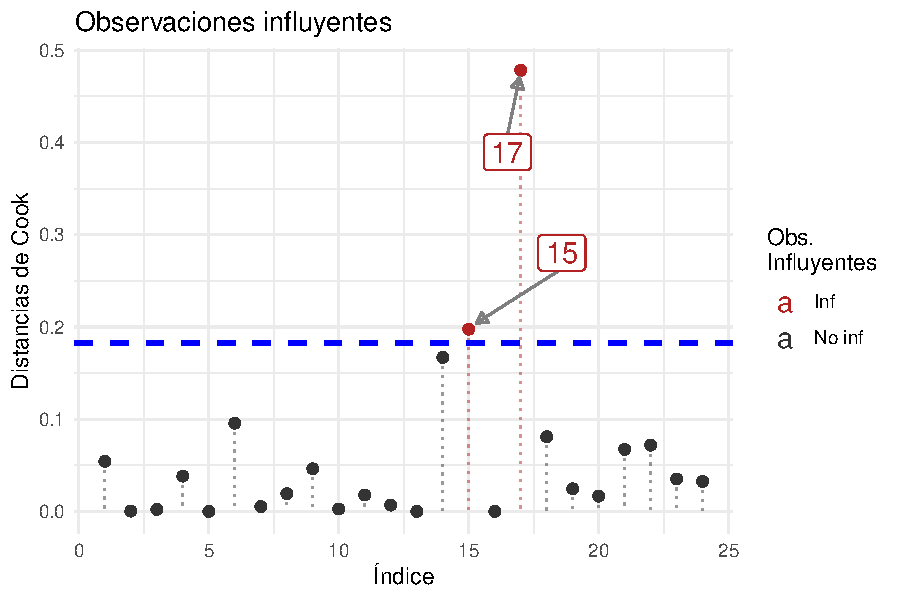
\includegraphics{diagnosticorrpp_files/figure-latex/observaciones influyentes para mejor modelo por BIC-1.pdf}
\caption{Evaluación de observaciones influyentes para el mejor modelo
por BIC}
\end{figure}

\end{document}
